\documentclass[12pt,a4paper]{article}
%\usepackage{fontspec, xunicode, xltxtra}  
%\setmainfont{Hiragino Sans GB}  
%\usepackage{xeCJK}
%\setCJKmainfont[BoldFont=STZhongsong, ItalicFont=STKaiti]{STSong}
%\setCJKsansfont[BoldFont=STHeiti]{STXihei}
%\setCJKmonofont{STFangsong}

%使用Xelatex编译

% 设置页面
%==================================================
\linespread{2} %行距
% \usepackage[top=1in,bottom=1in,left=1.25in,right=1.25in]{geometry}
% \headsep=2cm
% \textwidth=16cm \textheight=24.2cm
%==================================================

% 其它需要使用的宏包
%==================================================
\usepackage[colorlinks,linkcolor=blue,anchorcolor=red,citecolor=green,urlcolor=blue]{hyperref} 
\usepackage{tabularx}
\usepackage{authblk}         % 作者信息
\usepackage{algorithm}     % 算法排版
\usepackage{amsmath}     % 数学符号与公式
\usepackage{amsfonts}     % 数学符号与字体
\usepackage{mathrsfs}      % 花体
\usepackage{amssymb}
\usepackage[framemethod=TikZ]{mdframed}

\usepackage{graphicx} 
\usepackage{graphics}
\usepackage{color}
\usepackage{xcolor}
\usepackage{tcolorbox}
\usepackage{lipsum}
\usepackage{empheq}

\usepackage{fancyhdr}       % 设置页眉页脚
\usepackage{fancyvrb}       % 抄录环境
\usepackage{float}              % 管理浮动体
\usepackage{geometry}     % 定制页面格式
\usepackage{hyperref}       % 为PDF文档创建超链接
\usepackage{lineno}          % 生成行号
\usepackage{listings}        % 插入程序源代码
\usepackage{multicol}       % 多栏排版
%\usepackage{natbib}         % 管理文献引用
\usepackage{rotating}       % 旋转文字,图形,表格
\usepackage{subfigure}    % 排版子图形
\usepackage{titlesec}       % 改变章节标题格式
\usepackage{moresize}   % 更多字体大小
\usepackage{anysize}
\usepackage{indentfirst}  % 首段缩进
\usepackage{booktabs}   % 使用\multicolumn
\usepackage{multirow}    % 使用\multirow

\usepackage{wrapfig}
\usepackage{titlesec}     % 改变标题样式
\usepackage{enumitem}
\usepackage{aas_macros}

\renewcommand{\vec}[1]{\boldsymbol{#1}}
\newcommand{\me}{\mathrm{e}}
\newcommand{\mi}{\mathrm{i}}
\newcommand{\dif}{\mathrm{d}}
\newcommand{\tabincell}[2]{\begin{tabular}{@{}#1@{}}#2\end{tabular}}

\def\kpc{{\rm kpc}}
\def\km{{\rm km}}
\def\cm{{\rm cm}}
\def\TeV{{\rm TeV}}
\def\GeV{{\rm GeV}}
\def\MeV{{\rm MeV}}
\def\GV{{\rm GV}}
\def\MV{{\rm MV}}
\def\yr{{\rm yr}}
\def\s{{\rm s}}
\def\ns{{\rm ns}}
\def\GHz{{\rm GHz}}
\def\muGs{{\rm \mu Gs}}
\def\arcsec{{\rm arcsec}}
\def\K{{\rm K}}
\def\microK{\mu{\rm K}}
\def\sr{{\rm sr}}
\newcolumntype{p}{D{,}{\pm}{-1}}

\renewcommand{\figurename}{Fig.}
\renewcommand{\tablename}{Tab.}

\renewcommand{\arraystretch}{1.5}

\setlength{\parindent}{0pt}  %取消每段开头的空格

\newcounter{theo}[section]\setcounter{theo}{0}
\renewcommand{\thetheo}{\arabic{section}.\arabic{theo}}
\newenvironment{theo}[2][]{%
\refstepcounter{theo}%
\ifstrempty{#1}%
{\mdfsetup{%
frametitle={%
\tikz[baseline=(current bounding box.east),outer sep=0pt]
\node[anchor=east,rectangle,fill=blue!20]
{\strut Theorem~\thetheo};}}
}%
{\mdfsetup{%
frametitle={%
\tikz[baseline=(current bounding box.east),outer sep=0pt]
\node[anchor=east,rectangle,fill=blue!20]
{\strut Theorem~\thetheo:~#1};}}%
}%
\mdfsetup{innertopmargin=10pt,linecolor=blue!20,%
linewidth=2pt,topline=true,%
frametitleaboveskip=\dimexpr-\ht\strutbox\relax
}
\begin{mdframed}[]\relax%
\label{#2}}{\end{mdframed}}

\newcommand*\widefbox[1]{\fbox{\hspace{2em}#1\hspace{2em}}}

\title{Nonlinear Equations}
\author{}
\date{\today}
\begin{document}

\maketitle

\section{Oscillations and the Sturm Separation Theorem}
\cite{george1991differential, simmons2016differential} What we can about the essential characteristics of the solutions of (\ref{eq:diff_equ}) by direct analysis of the equation itself, in the absence of formal expressions for these solutions. 
\begin{equation}
y^{\prime \prime} +P(x) y^\prime +Q(x) y = 0 ~.
\label{eq:diff_equ}
\end{equation}
Many properties of the solutions of a differential equation can be discovered by studying the equation itself, without
solving it in any traditional sense. Consider the equation
\begin{equation}
y^{\prime \prime}  + y = 0 ~.
\label{eq:sin_equ}
\end{equation}
$y_1(x)= \sin x$ and $y_2(x) =\cos x$ are two linearly independent solutions of (\ref{eq:sin_equ}); that they are fully determined by the initial conditions \textcolor{blue}{$y_1(0) = 0$}, \textcolor{blue}{$y_1^\prime(0) = 1$} and \textcolor{blue}{$y_2(0) = 1$}, \textcolor{blue}{$y_2^\prime(0) = 0$}; and that the general solution is $y(x) = c_1y_1(x)+c_2y_2(x)$. 

Let \textcolor{blue}{$y = s(x)$} be defined as the solution of (\ref{eq:sin_equ}) determined by the initial conditions \textcolor{blue}{$s(0) = 0$} and \textcolor{blue}{$s^\prime(0) = 1$}. If we try to sketch the graph of $s(x)$ by letting $x$ increase from $0$, the initial conditions tell us to start the curve at the origin and let it rise with slope beginning at $1$ (Figure \ref{fig:sin_func}). From the equation itself we have $s^{\prime \prime}(x) = -s(x)$, so when the curve is above the $x$-axis, $s^{\prime \prime}(x)$ is a negative number that increases in magnitude as the curve rises. Since $s^{\prime \prime}(x)$ is the rate of change of the slope $s^{\prime}(x)$, this \textcolor{blue}{slope decreases at an increasing rate as the curve lifts}, and it must \textcolor{blue}{reach $0$ at some point $x = m$}. As \textcolor{blue}{$x$ continues to increase}, the \textcolor{blue}{curve falls toward the $x$-axis}, \textcolor{blue}{$s^{\prime}(x)$ decreases at a decreasing rate}, and the \textcolor{blue}{curve crosses the $x$-axis at a point} we can define to be $\pi$. Since $s^{\prime \prime}(x)$ depends only on $s(x)$, we see that the graph between $x = 0$ and $x = \pi$ is symmetric about the line $x = m$, so $m = \pi/2$ and $s^{\prime}(\pi) = -1$. A similar argument shows that the next portion of the curve is an inverted replica of the first arch, and so on indefinitely.

%===========================================================================================================================
\begin{figure*}
\centering
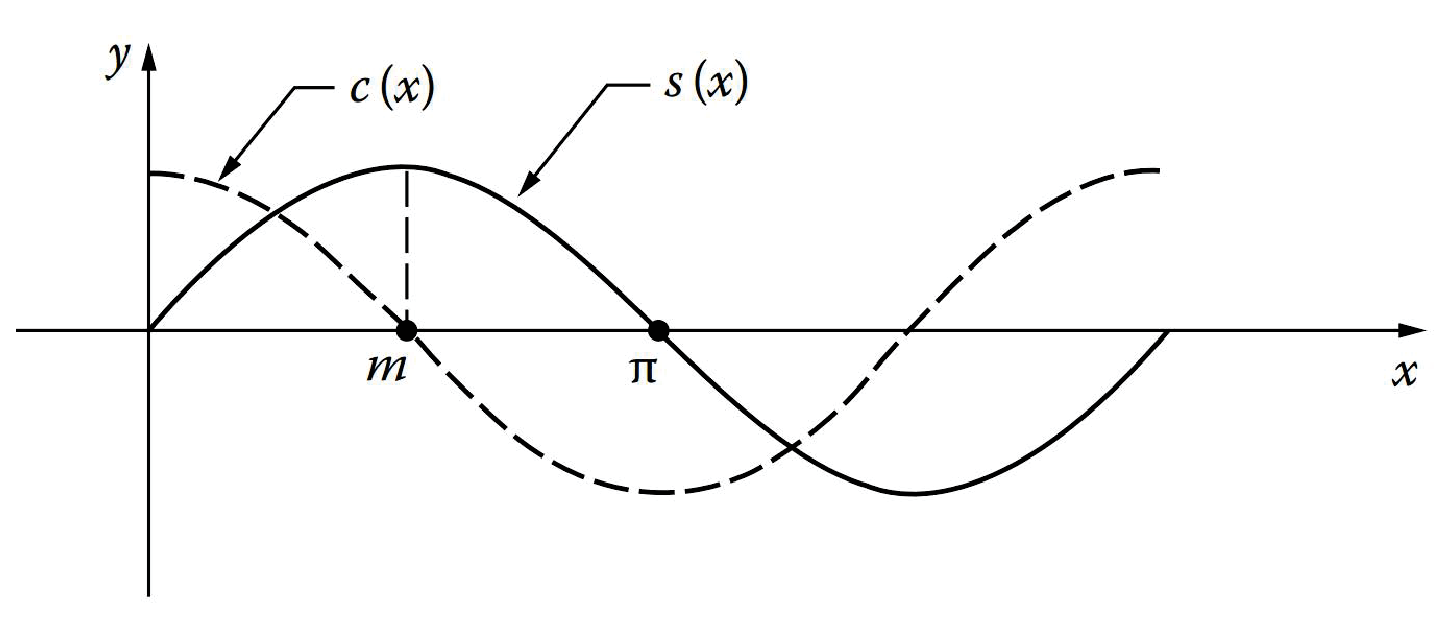
\includegraphics[height=6.cm, angle=0]{sin_func.eps}
\caption{
}
\label{fig:sin_func}
\end{figure*}
%===========================================================================================================================

Introduce \textcolor{blue}{$y = c(x)$} as the solution of (\ref{eq:sin_equ}) determined by the initial conditions \textcolor{blue}{$c(0) = 1$} and \textcolor{blue}{$c^\prime(0) = 0$}. The graph of $c(x)$ starts at the point $(0, 1)$ and moves to the right with slope beginning at $0$(Figure \ref{fig:sin_func}). Since by equation (\ref{eq:sin_equ}) $c^{\prime \prime}(x) = -c(x)$, the same reasoning as before shows that the curve bends down and crosses the $x$-axis. It is natural to conjecture that the height of the first arch of $s(x)$ is $1$, that the first zero of $c(x)$ is $\pi/2$, etc.; but to establish these guesses as facts, we begin by showing that
\begin{align}
s^\prime(x) &= c(x) ~, \\
c^\prime(x) &= -s(x) ~.
\label{dsin_cos}
\end{align}
Equ. (\ref{eq:sin_equ}) yields $y^{\prime \prime \prime}+ y^{\prime} = 0$ or $(y^{\prime })^{\prime \prime}+y^{\prime} = 0$, so the \textcolor{blue}{derivative of any solution of (\ref{eq:sin_equ}) is again a solution}. Thus $s^\prime(x)$ and $c(x)$ are both solutions of (\ref{eq:sin_equ}) and they \textcolor{blue}{have the same values and the same derivatives at $x = 0$}. This follows at once from $s^\prime(0) = 1$, $c(0) = 1$ and $s^{\prime \prime}(0) = -s(0) = 0$, $c^{\prime }(0) = 0$. The formula (\ref{dsin_cos}) is an immediate consequence of the first, for $c^{\prime}(x) = s^{\prime\prime}(x) = -s(x)$. Now use (\ref{dsin_cos}) to prove
\begin{equation}
s(x)^2 +c(x)^2 = 1 ~.
\label{eq:s2pc2e1}
\end{equation}
Since the derivative of the left side of (\ref{eq:s2pc2e1}) is
\begin{equation}
2 s(x) c(x) - 2c(x) s(x) ~,
\end{equation}
which is $0$. $s(x)^2 +c(x)^2$ equals a constant, and this constant must be $1$ because $s(0)^2 +c(0)^2 = 1$. It follows at once from (\ref{eq:s2pc2e1}) that the height of the first arch of $s(x)$ is $1$ and that the first zero of $c(x)$ is $\pi/2$. This result also enables us to show that $s(x)$ and $c(x)$ are linearly independent, for their Wronskian is
\begin{equation*}
W[s(x), c(x)] = s(x) c^\prime(x) - c(x) s^\prime(x) = -s(x)^2 -c(x)^2 = -1 ~.
\end{equation*}
\begin{align}
s(x+a) &= s(x)c(a) +c(x)s(a) ~, \\
c(x+a) &= c(x)c(a) -s(x)s(a) ~, \\
s(2x) &= 2s(x) c(x) ~, \\
c(2x) &= c(x)^2 -s(x)^2 ~, \\
s(x+2\pi) &= s(x) ~, \\
c(x+2\pi) &= c(x) ~.
\end{align}
From the above results that the positive zeros of $s(x)$ and $c(x)$ are, respectively, $\pi, 2\pi, 3\pi, \cdots$ and $\pi/2, \pi/2 + \pi, \pi/2 + 2\pi, \cdots$.

First, we have extracted almost every significant property of the functions $\sin x$ and $\cos x$ from equation (\ref{eq:sin_equ}) by the methods of differential equations alone, without using any prior knowledge of trigonometry. Second, the tools we did use consisted chiefly of convexity arguments (involving the sign and magnitude of the second derivative) and the basic properties of linear equations. 




\begin{tcolorbox}[colback=green!5,colframe=green!40!black,title= Theorem A]
If $y_1(x)$ and $y_2(x)$ are two linearly independent solutions of
\begin{equation}
y^{\prime \prime} +P(x) y^\prime +Q(x) y = 0 ~.
\end{equation}
then the \textcolor{red}{zeros of these functions are distinct and occur alternately} --- in the sense that $y_1(x)$ vanishes exactly once between any two successive zeros of $y_2(x)$, and conversely.
\end{tcolorbox}
It is called \textcolor{red}{Sturm separation theorem}.


\begin{tcolorbox}[colback=green!5,colframe=green!40!black,title= Theorem B]
If \textcolor{red}{$q(x) < 0$}, and if $u(x)$ is a nontrivial solution of $u^{\prime \prime} +q(x) u = 0$, then \textcolor{red}{$u(x)$ has at most one zero}.
\end{tcolorbox}


\begin{tcolorbox}[colback=green!5,colframe=green!40!black,title= Theorem C]
Let $u(x)$ be any nontrivial solution of $u^{\prime \prime}+q(x)u = 0$, where \textcolor{red}{$q(x) > 0$ for all $x > 0$}. If
\begin{equation}
\color{red} \int_1^\infty q(x) \dif x = \infty ~,
\end{equation}
then $u(x)$ has \textcolor{red}{infinitely many zeros on the positive $x$-axis}.
\end{tcolorbox}






\section{The Sturm Comparison Theorem}
\cite{george1991differential, simmons2016differential} Consider the oscillation behavior of nontrivial
solutions of the differential equation
\begin{equation}
y^{\prime \prime} +q(x) y = 0 ~,
\label{eq:sturm_cmp}
\end{equation}
where \textcolor{red}{$q(x)$ is a positive function}. We begin with a theorem that rules out the possibility of infinitely many oscillations on closed intervals. 
\begin{tcolorbox}[colback=green!5,colframe=green!40!black,title= Theorem A]
Let $y(x)$ be a nontrivial solution of equation (\ref{eq:sturm_cmp}) on a \textcolor{red}{closed interval $[a, b]$}. Then $y(x)$ has \textcolor{red}{at most a finite number of zeros in this interval}.
\end{tcolorbox}









\begin{tcolorbox}[colback=green!5,colframe=green!40!black,title= Theorem B]
Let $y(x)$ and $z(x)$ be nontrivial solutions of
\begin{equation}
y^{\prime \prime} +q(x) y = 0 ~,
\end{equation}
and
\begin{equation}
z^{\prime \prime} +r(x) z = 0 ~,
\end{equation}
where $q(x)$ and $r(x)$ are \textcolor{red}{positive functions} such that \textcolor{red}{$q(x) > r(x)$}. Then \textcolor{red}{$y(x)$ vanishes at least once between any two successive zeros of $z(x)$}.
\end{tcolorbox}


\begin{tcolorbox}[colback=green!5,colframe=green!40!black,title= Theorem C]
Let $y_p(x)$ be a nontrivial solution of Bessel's equation on the positive $x$-axis. If \textcolor{red}{$0 \leqslant p < 1/2$}, then every interval of length $\pi$ contains \textcolor{red}{at least one zero} of $y_p(x)$; if \textcolor{red}{$p = 1/2$}, then the \textcolor{red}{distance between successive zeros of $y_p(x)$ is exactly $\pi$}; and if \textcolor{red}{$p > 1/2$}, then \textcolor{red}{every interval of length $\pi$ contains at most one zero of $y_p(x)$}.
\end{tcolorbox}

















\section{Autonomous Systems. The Phase Plane and Its Phenomena}
\cite{george1991differential, simmons2016differential} The second order nonlinear equations of the form
\begin{equation}
\dfrac{\dif^2 x}{\dif t^2} = f\left(x, \dfrac{\dif x}{\dif t} \right) ~.
\label{eq:nonlinear}
\end{equation}
If we imagine a simple dynamical system consisting of a particle of unit mass moving on the $x$-axis, and if $f(x, \dif x/\dif t)$ is the force acting on it, then Eq. (\ref{eq:nonlinear}) is the equation of motion. The values of $x$ (position) and $\dif x/\dif t$ (velocity), which at each instant characterize the state of the system, are called its \textcolor{red}{phases}, and the \textcolor{orange}{plane of the variables $x$ and $\dif x/\dif t$} is called the \textcolor{red}{phase plane}. Introduce the variable \textcolor{orange}{$y = \dif x/\dif t$},
\begin{equation}
\left\{
\begin{aligned}
\dfrac{\dif x}{\dif t} & =  y \\
\dfrac{\dif y}{\dif t} & =  f(x, y) ~.
\end{aligned}
\label{eq:system}
\right.
\end{equation}
When \textcolor{blue}{$t$ is regarded as a parameter}, then in general \textcolor{blue}{a solution is a pair of functions $x(t)$ and $y(t)$ defining a curve in the $xy$-plane}, which is simply the \textcolor{blue}{phase plane}.

More general systems of the form are
\begin{equation}
\color{red}
\left\{
\begin{aligned}
\dfrac{\dif x}{\dif t} & =  F(x,y) \\
\dfrac{\dif y}{\dif t} & =  G(x, y) ~.
\label{eq:system_gen}
\end{aligned}
\right.
\end{equation}
where \textcolor{blue}{$F$} and \textcolor{blue}{$G$} are \textcolor{blue}{continuous} and have \textcolor{blue}{continuous first partial derivatives throughout the plane}. A system of this kind, in which the \textcolor{yellow}{independent variable $t$ does not appear in the functions $F$ and $G$} on the right, is said to be \textcolor{yellow}{autonomous}.

If $t_0$ is any number and $(x_0,y_0)$ is any point in the phase plane, then there exists a \textcolor{blue}{unique solution}
\begin{equation}
\left\{
\begin{aligned}
x & = x(t) \\
y & =  y(t) ~.
\label{eq:system_sol}
\end{aligned}
\right.
\end{equation}
of Eq. (\ref{eq:system_gen}) such that $x(t_0) = x_0$ and $y(t_0) = y_0$. If $x(t)$ and $y(t)$ are not both constant functions, Eq. (\ref{eq:system_sol}) defines \textcolor{red}{a curve in the phase plane} called \textcolor{red}{a path (trajectory and characteristic) of the system}.

If Eqs. (\ref{eq:system_sol}) is a solution of Eqs. (\ref{eq:system_gen}), then
\begin{equation}
\left\{
\begin{aligned}
x & = x(t+\color{red}{c}) \\
y & = y(t+\color{red}{c}) ~.
\label{eq:w_c}
\end{aligned}
\right.
\end{equation}
is also a solution for any constant \textcolor{red}{$c$}. \textcolor{orange}{Each path is represented by many solutions}, which \textcolor{orange}{differ from one another only by a translation of the parameter}. Any path through the point $(x_0,y_0)$ must correspond to a solution of the form (\ref{eq:w_c}). It follows from this that \textcolor{blue}{at most one path passes through each point of the phase plane}. Furthermore, the \textcolor{blue}{direction of increasing $t$ along a given path is the same for all solutions representing the path}. A path is a directed curve, and use arrows to indicate the direction in which the path is traced out as $t$ increases. The \textcolor{blue}{paths of (\ref{eq:system_gen}) cover the entire phase plane and do not intersect one another}. The only exceptions to this statement occur at points $(x_0,y_0)$ where both $F$ and $G$ vanish:
\begin{align*}
\color{red} F(x_0, y_0) = 0 ~, \\
\color{red} G(x_0, y_0) = 0 ~.
\end{align*}
These points are called \textcolor{red}{critical points}, and \textcolor{blue}{at such a point the unique solution is the constant solution $x=x_0$ and $y=y_0$}. A constant solution does not define a path, and therefore no path goes through a critical point. We will always assume that \textcolor{yellow}{each critical point $(x_0,y_0)$ is isolated}, i.e.  there \textcolor{yellow}{exists a circle centered on $(x_0,y_0)$ that contains no other critical point}.

Consider the autonomous system (\ref{eq:system}) arising from the dynamical equation (\ref{eq:nonlinear}). In this case a critical point is a point $(x_0,0)$ at which $y=0$ and $f(x_0,0)=0$; that is, it corresponds to a state of the particle's motion in which both the velocity $\dif x/\dif t$ and the acceleration $\dif y/\dif t = \dif^2 x/\dif t^2$ vanish. This means that the particle is at rest with no force acting on it, and is therefore in a state of equilibrium.


Consider Figure (\ref{fig:phase_plane}) and the \textcolor{blue}{two-dimensional vector field} defined by
\begin{equation}
\vec{V}(x,y) = F(x,y) \vec{i} + G(x,y) \vec{j} ~,
\end{equation}
which at a typical point $P=(x,y)$ has horizontal component $F(x,y)$ and vertical component $G(x,y)$. Since $\dif x/\dif t= F$ and $\dif y/\dif t = G$, this vector is tangent to the path at $P$ and points in the direction of increasing $t$. If we think of $t$ as time, then $V$ can be interpreted as the velocity vector of a particle moving along the path. We can also imagine that the entire phase plane is filled with particles, and that each path is the trail of a moving particle preceded and followed by many others on the same path and accompanied by yet others on nearby paths. This situation can be described as a two-dimensional fluid motion; and since the \textcolor{green}{system (\ref{eq:system_gen}) is autonomous}, which means that the \textcolor{green}{vector $\vec{V}(x,y)$ at a fixed point $(x,y)$ does not change with time}, the \textcolor{green}{fluid motion is stationary}. The paths are the trajectories of the moving particles, and the critical points $Q$, $R$, and $S$ are points of zero velocity where the particles are at rest (i.e., stagnation points of the fluid motion).

The most striking features of the fluid motion illustrated in Figure (\ref{fig:phase_plane}) are: \\
(a) the critical points; \\
(b) the arrangement of the paths near critical points; \\
(c) the stability or instability of critical points, that is, whether a particle near such a point remains near or wanders off into another part of the plane; \\
(d) closed paths (like $C$ in the figure), which correspond to periodic solutions.

These features constitute a major part of the \textcolor{red}{phase portrait} (or overall picture of the paths) of the system (\ref{eq:system_gen}).  Since in general nonlinear equations and systems cannot be solved explicitly, the purpose of the qualitative theory is to \textcolor{green}{discover as much as possible about the phase portrait directly from the functions $F$ and $G$}. If $x(t)$ is a periodic solution of the dynamical equation (\ref{eq:nonlinear}), then its derivative $y(t)= \dif x/\dif t$ is also periodic and the corresponding path of the system (\ref{eq:system}) is closed. Conversely, if any path of (\ref{eq:system}) is closed, then (\ref{eq:nonlinear}) has a periodic solution. 





%===========================================================================================================================
\begin{figure*}
\centering
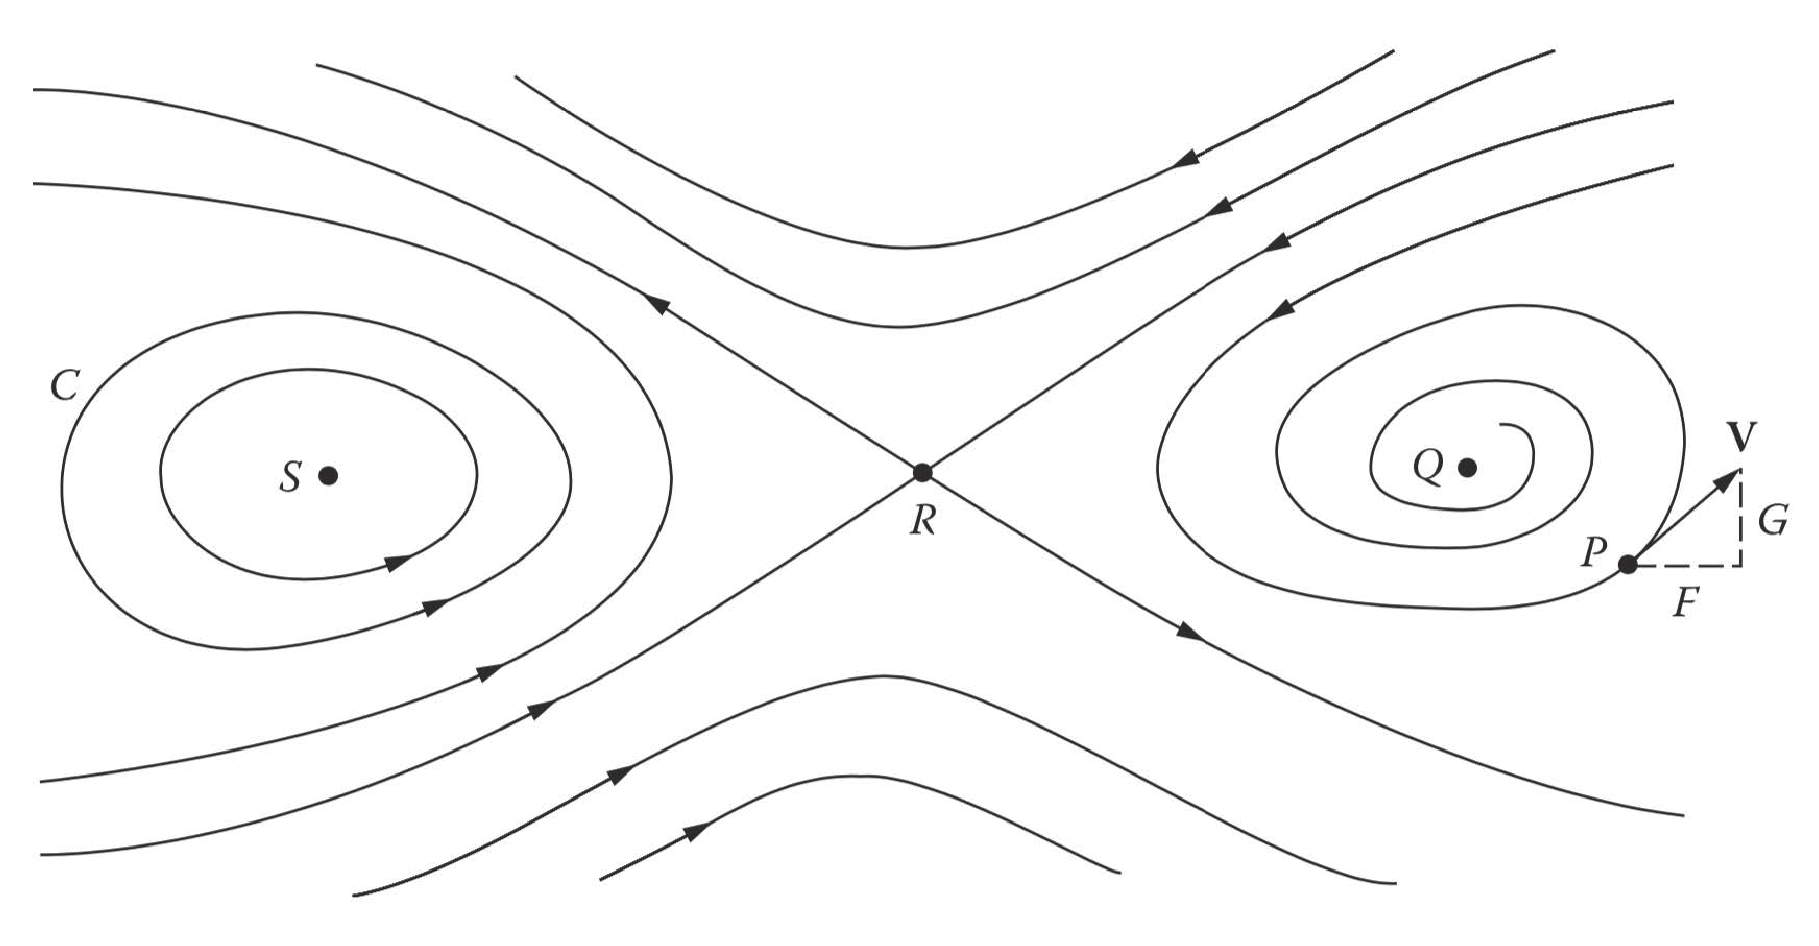
\includegraphics[height=6.cm, angle=0]{phase_plane.eps}
\caption{
}
\label{fig:phase_plane}
\end{figure*}
%===========================================================================================================================



\subsection{Autonomous First-Order Equations}
\cite{Herman:1742872} A first-order autonomous equation is given in the form
\begin{equation}
\dfrac{\dif y}{\dif t}  = f(y) ~.
\label{eq:first_auto}
\end{equation}
We assume $f$ and $\dfrac{\partial f}{\partial t}$ are continuous functions of $y$, thus the solutions of initial value problems exist and are unique.

A solution $y(t)$ of Equation (\ref{eq:first_auto}) is called an \textcolor{red}{equilibrium solution}, or a \textcolor{red}{fixed point solution}, if it is a constant solution satisfying $y^\prime(t) = 0$. Such solutions are the roots of the right-hand side of the differential equation $f(y) = 0$.





























\section{Types of Critical Points. Stability}
\cite{george1991differential, simmons2016differential} Consider an autonomous system
\begin{equation}
\left\{
\begin{aligned}
\dfrac{\dif x}{\dif t} & =  F(x,y) \\
\dfrac{\dif y}{\dif t} & =  G(x, y) ~.
\end{aligned}
\right.
\end{equation}
We assume that the functions $F$ and $G$ are continuous and have continuous first partial derivatives throughout the $xy$-plane. The critical points can be found in principle by solving the simultaneous equations $F(x,y)=0$ and $G(x,y)=0$. There are four simple types of critical points that occur quite frequently.

Let $(x_0,y_0)$ be an isolated critical point of (\ref{eq:nonlinear_gen}). If $C=[x(t),y(t)]$ is a path of (\ref{eq:nonlinear_gen}), then we say that $C$ approaches $(x_0,y_0)$ as $t \rightarrow \infty$ if
\begin{equation}
\lim_{t\rightarrow \infty} x(t) = x_0 ~, \\
\lim_{t\rightarrow \infty} y(t) = y_0\footnote{It can be proved that if Eqs. (\ref{eq:xy_limit}) is true for some solution $x(t)$, $y(t)$, then $(x_0, y_0)$ is necessarily a critical point.} ~.
\label{eq:xy_limit}
\end{equation}
Geometrically, this means that if $P = (x,y)$ is a point that traces out $C$ in accordance with the equations $x=x(t)$ and $y=y(t)$, then $P \rightarrow (x_0,y_0)$ as $t \rightarrow \infty$. If it is also true that
\begin{equation}
\lim_{t\rightarrow \infty} \dfrac{y(t) -y_0}{x(t) -x_0}
\label{eq:quotient}
\end{equation}
exists, or if the quotient in (\ref{eq:quotient}) becomes either positively or negatively infinite as $t \rightarrow \infty$, then we say that $C$ enters the critical point $(x_0,y_0)$ as $t \rightarrow \infty$. The quotient in (\ref{eq:quotient}) is the slope of the line joining $(x_0,y_0)$ and the point $P$ with coordinates $x(t)$ and $y(t)$, so the additional requirement means that this line approaches a definite direction as $t \rightarrow \infty$. In the above definitions, we may also consider limits as $t \rightarrow -\infty$. These properties are properties of the path $C$, and do not depend on which solution is used to represent this path.

In most cases, however, to find the paths it is necessary to eliminate $t$ between the two equations of the system, which yields
\begin{equation}
\dfrac{\dif y}{\dif x} = \dfrac{G(x,y)}{F(x,y)} ~.
\label{eq:tangent}
\end{equation}
This first order equation gives the slope of the tangent to the path of (\ref{eq:nonlinear_gen}) that passes through the point $(x,y)$, provided that the functions $F$ and $G$ are not both zero at this point. In this case, of course, the point is a critical point and no path passes through it. The paths of (\ref{eq:nonlinear_gen}) coincide with the one-parameter family of integral curves of (\ref{eq:tangent}). While the paths of (\ref{eq:nonlinear_gen}) are directed curves, the integral curves of (\ref{eq:tangent}) have no direction associated with them.

\textbf{Nodes}. A critical point like that in Figure (\ref{fig:node}) is called a \textcolor{red}{node}. Such a point is approached and also entered by each path as $t \rightarrow \infty$ (or as $t \rightarrow -\infty$). For the node shown in Figure (\ref{fig:node}), there are four half-line paths, $AO$, $BO$, $CO$, and $DO$, which together with the origin make up the lines $AB$ and $CD$. All other paths resemble parts of parabolas, and as each of these paths approaches $O$ its slope approaches that of the line $AB$.

%===========================================================================================================================
\begin{figure*}
\centering
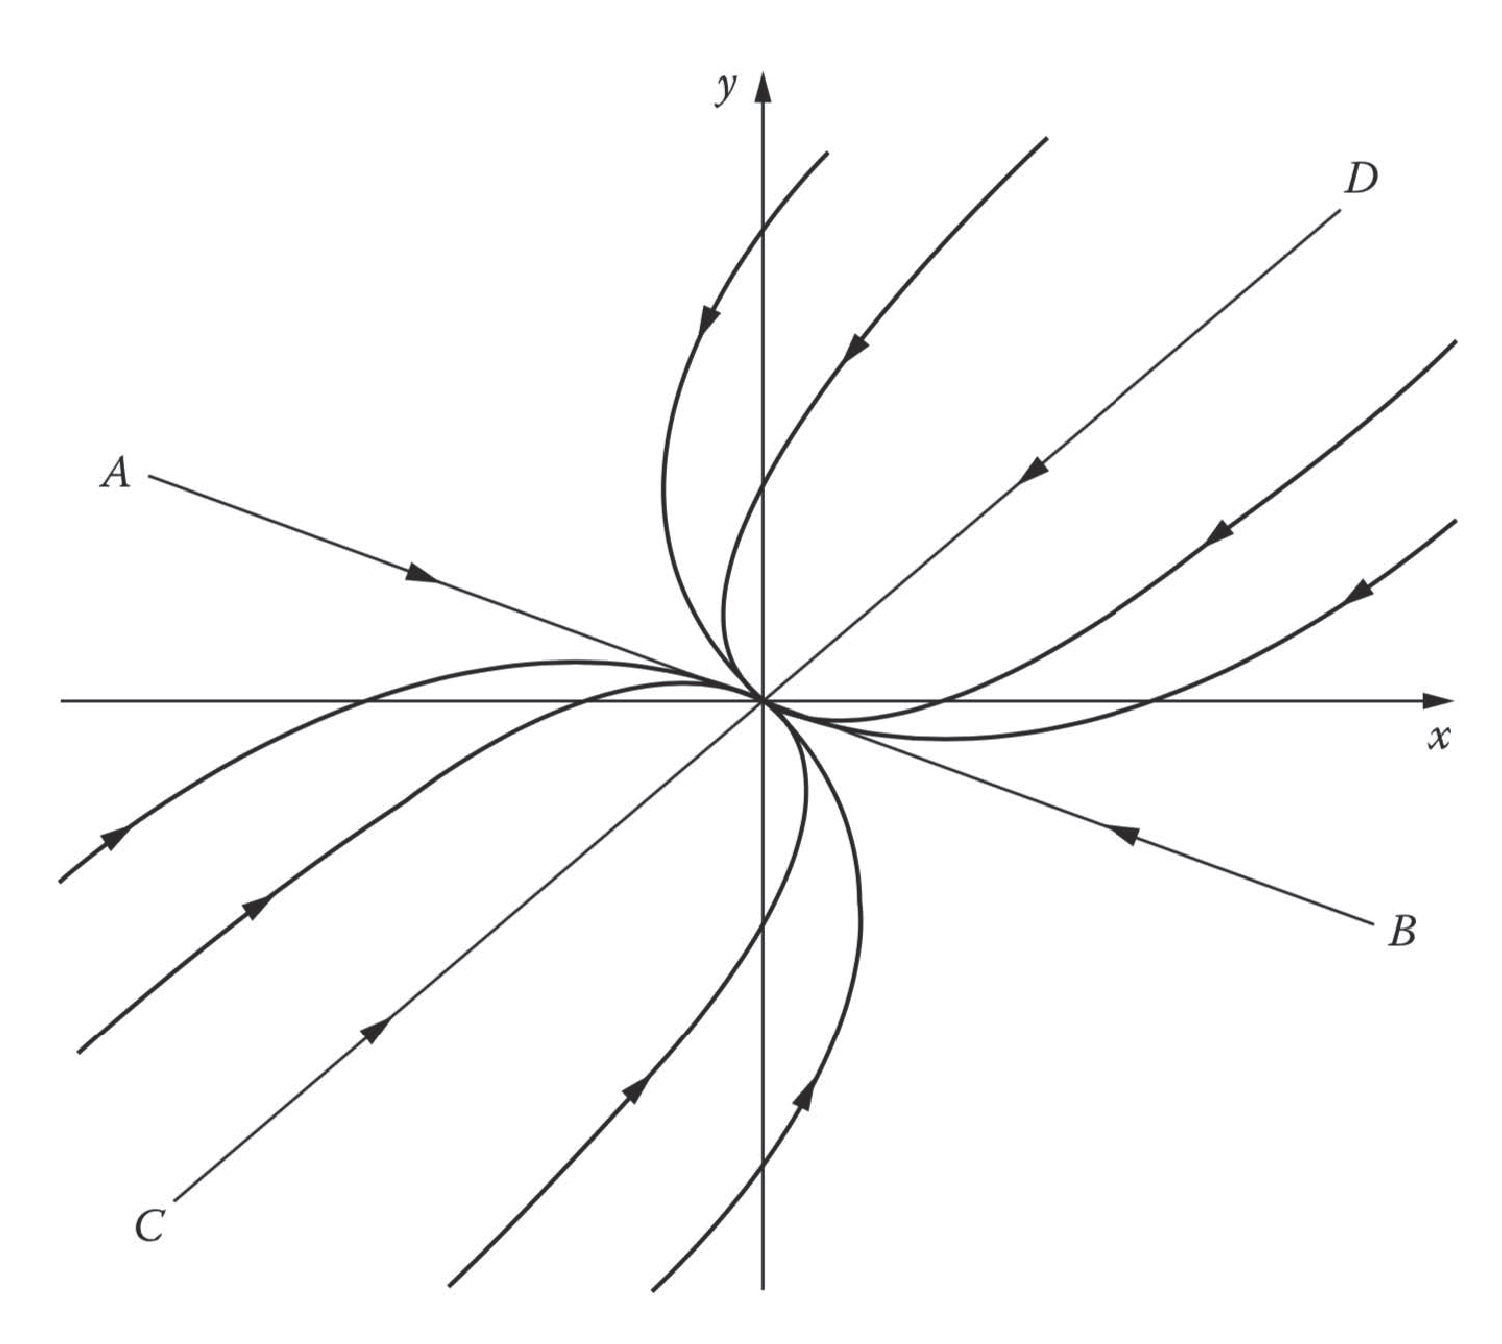
\includegraphics[height=9.cm, angle=0]{node.eps}
\caption{
}
\label{fig:node}
\end{figure*}
%===========================================================================================================================

\textbf{Saddle points}. A critical point like that in Figure (\ref{fig:saddle}) is called a \textcolor{red}{saddle point}. It is approached and entered by two half-line paths $AO$ and $BO$ as $t \rightarrow \infty$, and these two paths lie on a line $AB$. It is also approached and entered by two half-line paths $CO$ and $DO$ at $t \rightarrow -\infty$, and these two paths lie on another line $CD$. Between the four half-line paths there are four regions, and each contains a family of paths resembling hyperbolas. These paths do not approach $O$ as $t \rightarrow \infty$ or as $t \rightarrow -\infty$, but instead are asymptotic to one or another of the half-line paths as $t \rightarrow \infty$ and as $t \rightarrow -\infty$.


\textbf{Centers}. A center (sometimes called a \textcolor{red}{vortex}) is a critical point that is surrounded by a family of closed paths. It is not approached by any path as $t \rightarrow \infty$ or as $t \rightarrow -\infty$.

\textbf{Spirals}. A critical point like that in Figure (\ref{fig:spiral}) is called a \textcolor{red}{spiral} (or sometimes a \textcolor{red}{focus}). Such a point is approached in a spiral-like manner by a family of paths that wind around it an infinite number of times as $t \rightarrow \infty$ (or as $t \rightarrow -\infty$).

while the paths approach $O$, they do not enter it. That is, a point $P$ moving along such a path approaches $O$ as $t \rightarrow \infty$ (or as $t \rightarrow -\infty$), but the line $OP$ does not approach any definite direction.

%===========================================================================================================================
\begin{figure*}
\centering
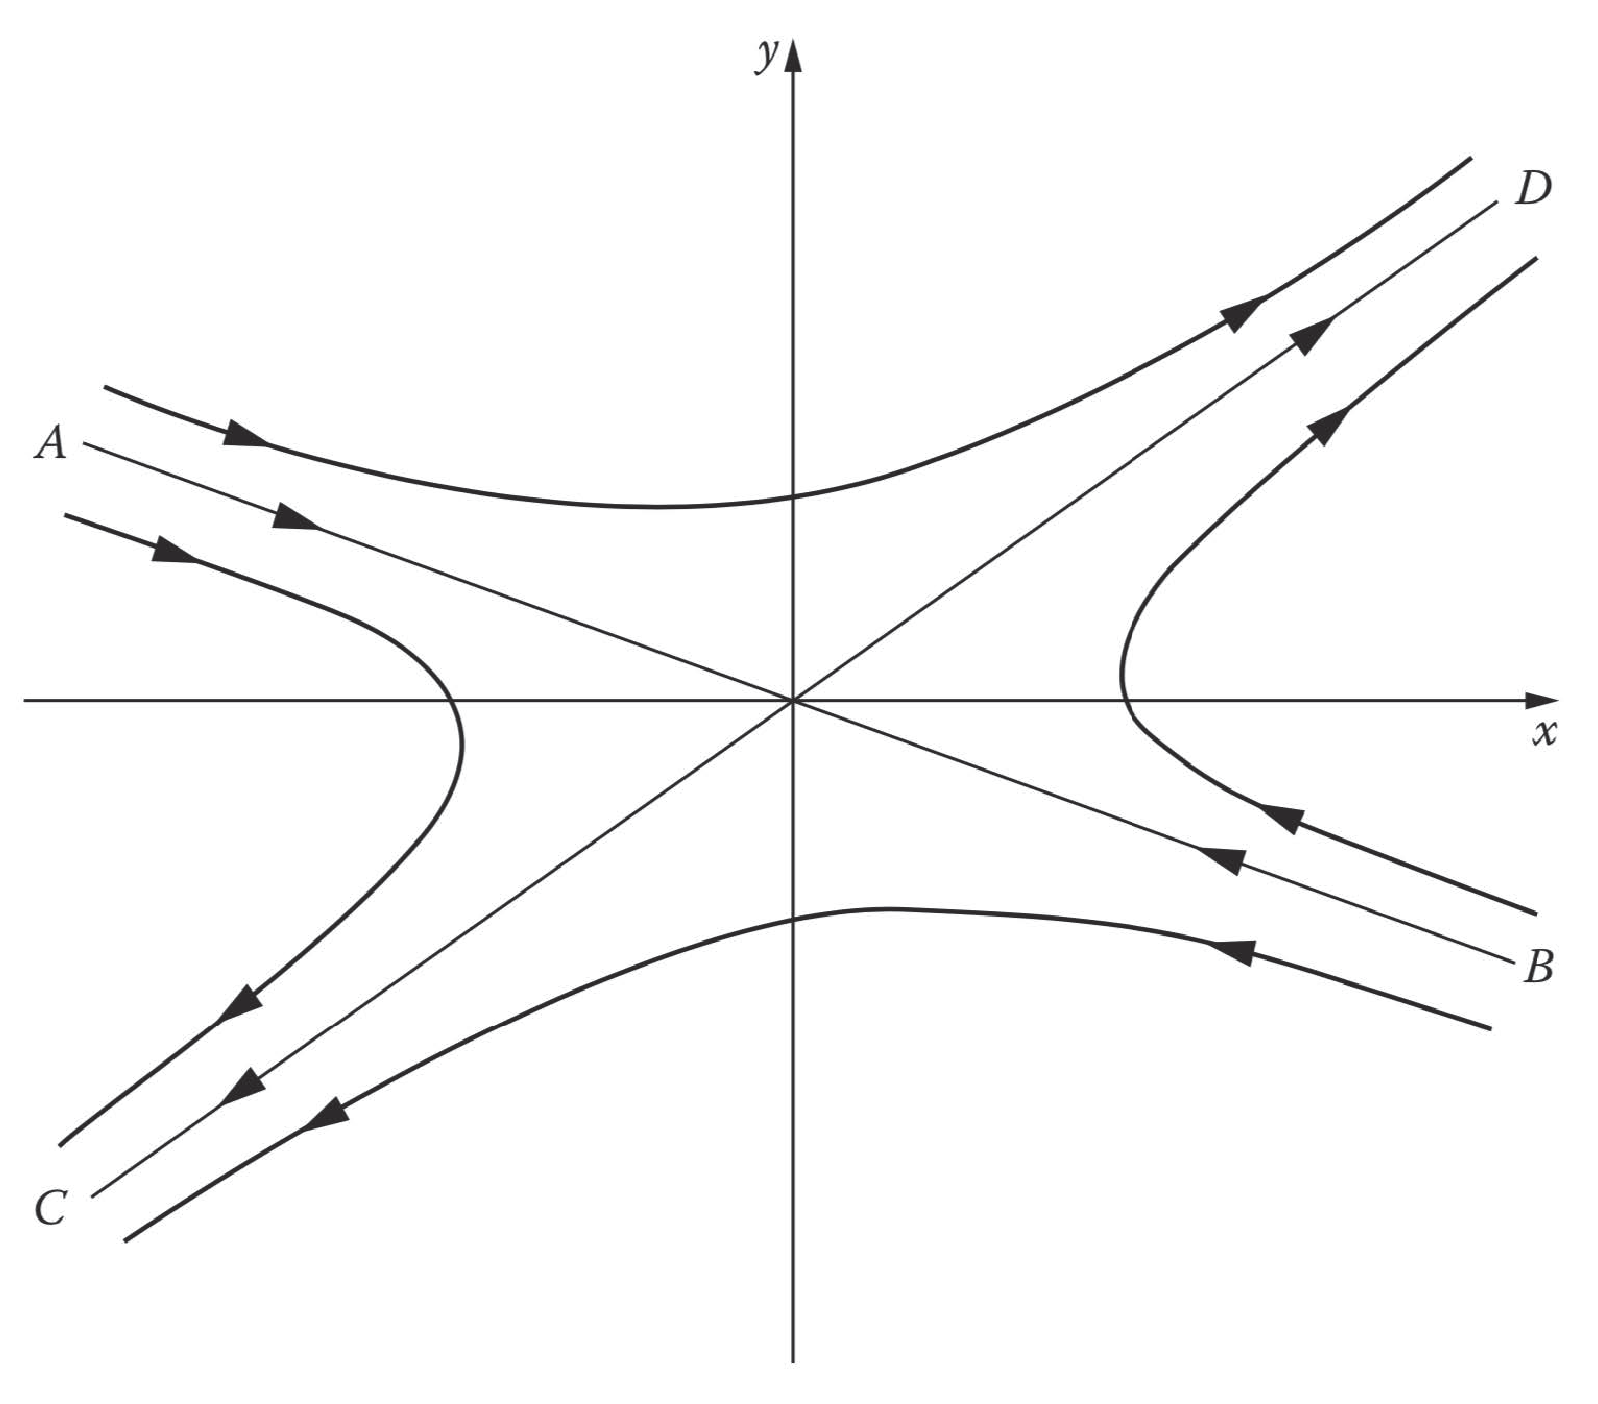
\includegraphics[height=9.cm, angle=0]{saddle.eps}
\caption{
}
\label{fig:saddle}
\end{figure*}
%===========================================================================================================================

%===========================================================================================================================
\begin{figure*}
\centering
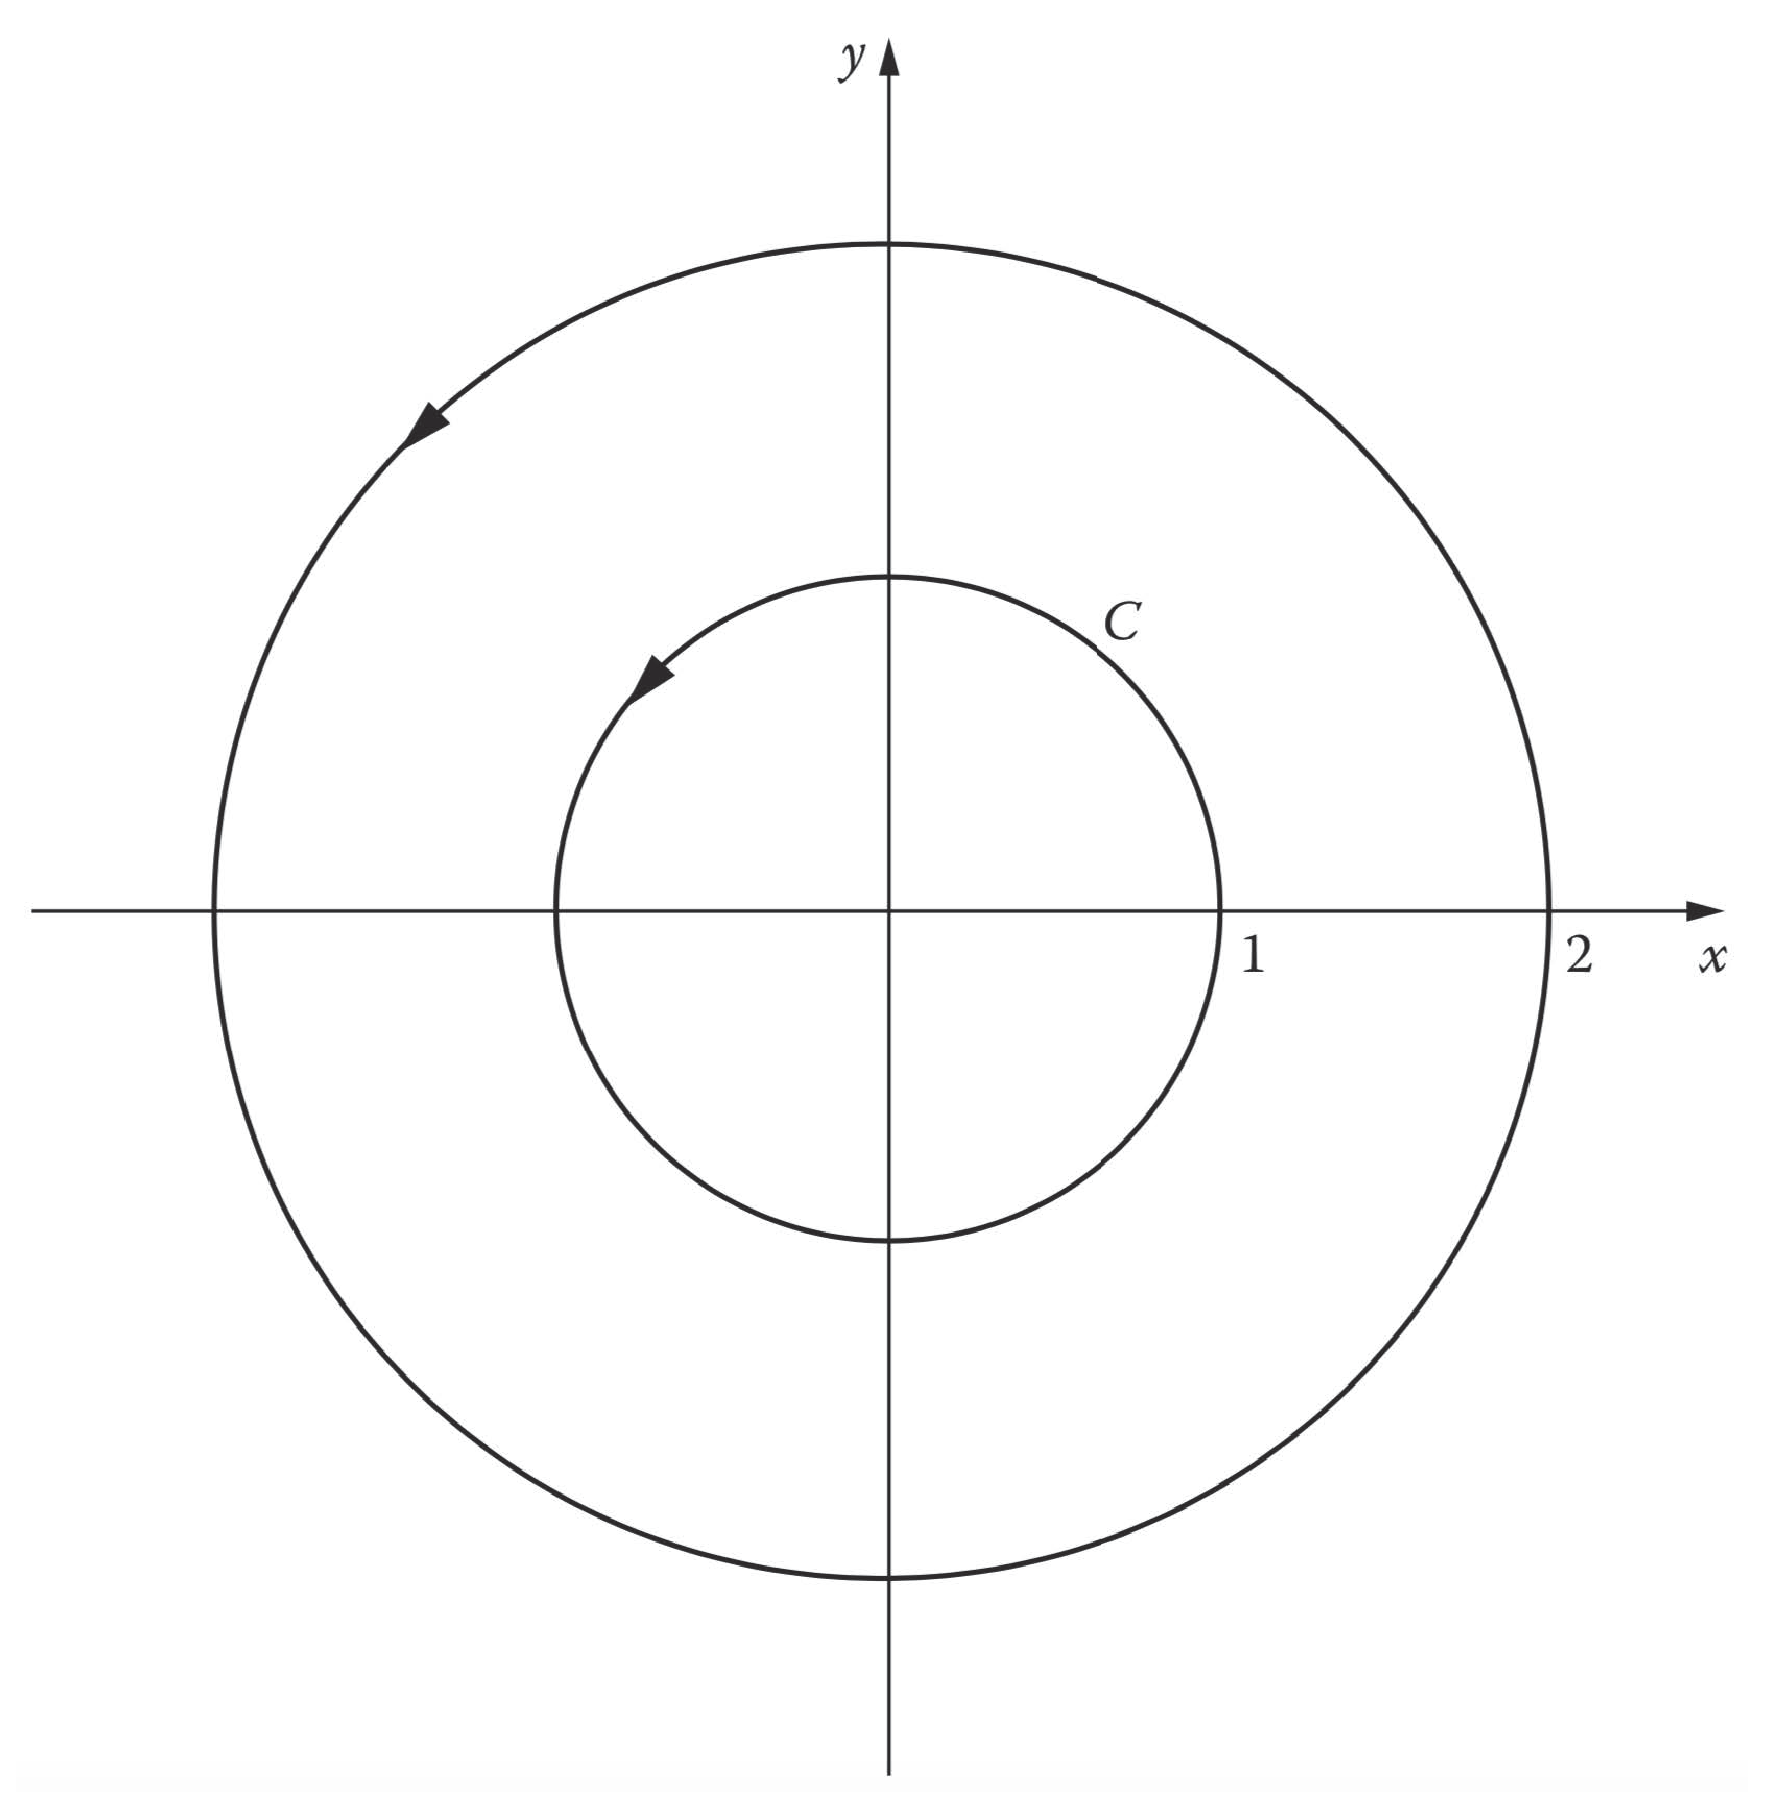
\includegraphics[height=9.cm, angle=0]{spiral.eps}
\caption{
}
\label{fig:spiral}
\end{figure*}
%===========================================================================================================================


A steady state has little physical significance unless it has a reasonable degree of permanence, i.e., unless it is stable. 

Consider an isolated critical point of the system (\ref{eq:nonlinear_gen}), and assume that this point is located at the origin $O=(0,0)$ of the phase plane. This critical point is said to be \textcolor{red}{stable} if for each positive number $R$ there exists a positive number $r \leqslant R$ such that every path which is inside the circle $x^2 +y^2 = r^2$ for some $t=t_0$ remains inside the circle $x^2 +y^2 =R^2$ for all $t > t_0$ (Figure \ref{fig:stable}). Loosely speaking, a critical point is stable if all paths that get sufficiently close to the point stay close to the point. Further, our critical point is said to be  \textcolor{red}{asymptotically stable} if it is stable and there exists a circle $x^2 + y^2 = r_0^2$ such that every path which is inside this circle for some $t = t_0$ approaches the origin as $t \rightarrow \infty$. If our critical point is not stable, then it is called \textcolor{red}{unstable}.

%===========================================================================================================================
\begin{figure*}
\centering
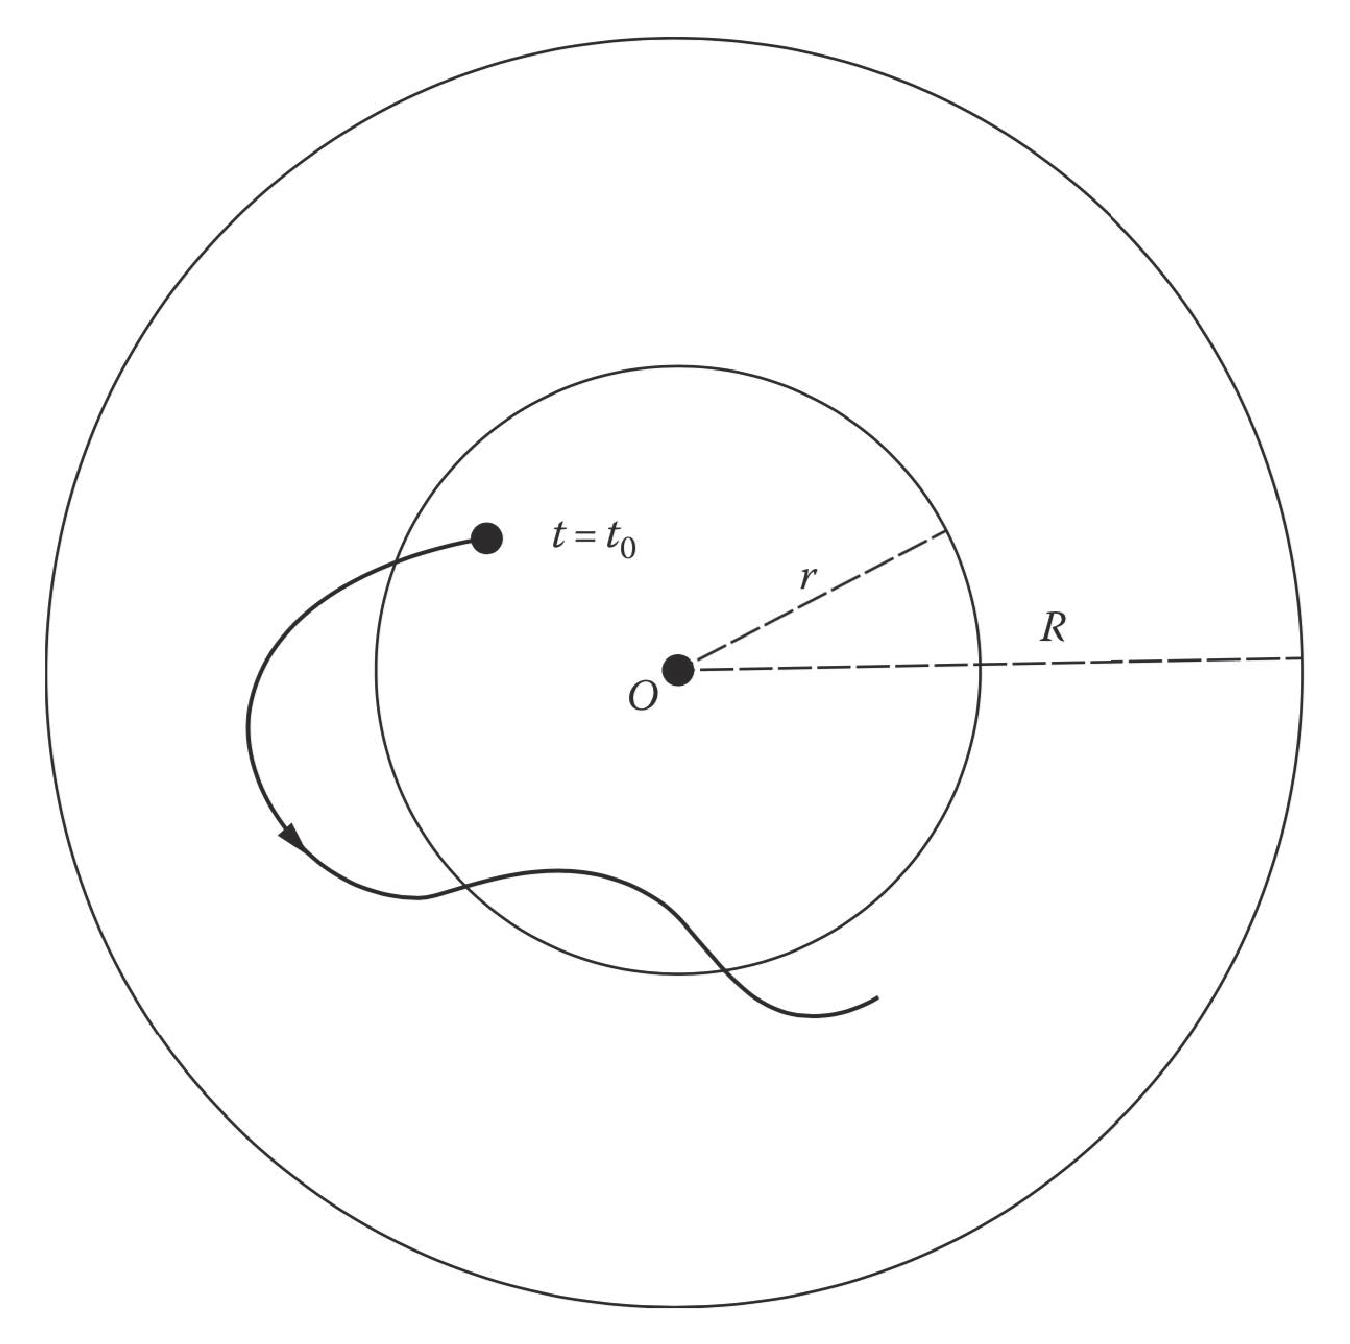
\includegraphics[height=9.cm, angle=0]{stable.eps}
\caption{
}
\label{fig:stable}
\end{figure*}
%===========================================================================================================================

\section{Critical Points and Stability for Linear Systems}
\cite{george1991differential, simmons2016differential} Study the phase portraits of nonlinear autonomous systems of the form
\begin{equation}
\left\{
\begin{aligned}
\dfrac{\dif x}{\dif t} & =  F(x,y) \\
\dfrac{\dif y}{\dif t} & =  G(x, y) ~.
\end{aligned}
\right.
\label{eq:nonlinear_gen}
\end{equation}





\section{Stability By Liapunov's Direct Method}
\cite{george1991differential, simmons2016differential} If the total energy of a physical system has a local minimum at a certain equilibrium point, then that point is stable. Consider an autonomous system
\begin{equation}
\left\{
\begin{aligned}
\dfrac{\dif x}{\dif t} & =  F(x,y) \\
\dfrac{\dif y}{\dif t} & =  G(x, y) ~.
\end{aligned}
\right.
\label{eq:nonlinear_gen}
\end{equation}
and assume that this system has an isolated critical point, which as usual we take to be the origin $(0,0)$\footnote{A critical point $(x_0,y_0)$ can always be moved to the origin by a simple translation of coordinates $\bar{x} = x - x_0$ and $\bar{y} = y - y_0$, so there is no loss of generality in assuming that it lies at the origin in the first place.}. Let $C = [x(t),y(t)]$ be a path of (\ref{eq:nonlinear_gen}), and consider a function $E(x,y)$ that is continuous and has continuous first partial derivatives in a region containing this path. If a point $(x,y)$ moves along the path in accordance with the equations $x = x(t)$ and $y = y(t)$, then $E(x,y)$ can be regarded as a function of $t$ along $C$ [we denote this function by $E(t)$] and its rate of change is
\begin{align}
\nonumber \dfrac{\dif E}{\dif t} &= \dfrac{\partial E}{\partial x} \dfrac{\dif x}{\dif t} + \dfrac{\partial E}{\partial y} \dfrac{\dif y}{\dif t} \\
&= \dfrac{\partial E}{\partial x} F + \dfrac{\partial E}{\partial y} G ~.
\label{eq:rofc}
\end{align}



A positive definite function $E(x,y)$ with the property that
\begin{equation}
\dfrac{\partial E}{\partial x} F + \dfrac{\partial E}{\partial y} G ~,
\label{eq:Liapunov_func}
\end{equation}
is negative semidefinite is called a \textcolor{red}{Liapunov function} for the system (\ref{eq:nonlinear_gen}). By formula (\ref{eq:rofc}), the requirement that (\ref{eq:Liapunov_func}) be negative semidefinite means that $\dif E/\dif t \leqslant 0$ - and therefore $E$ is nonincreasing - along the paths of (\ref{eq:nonlinear_gen}) near the origin. These functions generalize the concept of the total energy of a physical system.


\begin{tcolorbox}[colback=green!5,colframe=green!40!black,title= Theorem A]
If there exists a Liapunov function $E(x,y)$ for the system (\ref{eq:nonlinear_gen}), then the critical point $(0,0)$ is stable. Furthermore, if this function has the additional property that the function (\ref{eq:Liapunov_func}) is negative definite, then the critical point $(0,0)$ is asymptotically stable.
\end{tcolorbox}





\begin{tcolorbox}[colback=green!5,colframe=green!40!black,title= Theorem B]
The function $E(x,y) = ax^2+bxy+cy^2$ is positive definite if and only if $a > 0$ and $b^2 - 4ac < 0$, and is negative definite if and only if $a < 0$ and $b^2 - 4ac < 0$.
If $y \neq 0$, we have
\end{tcolorbox}


\section{Simple Critical Points of Nonlinear Systems}
\cite{george1991differential, simmons2016differential} Consider an autonomous system
\begin{equation*}
\left\{
\begin{aligned}
\dfrac{\dif x}{\dif t} & =  F(x,y) \\
\dfrac{\dif y}{\dif t} & =  G(x, y) ~.
\end{aligned}
\right.
\label{eq:nonlinear_gen}
\end{equation*}
with an isolated critical point at $(0,0)$. If $F(x,y)$ and $G(x,y)$ can be expanded in power series in $x$ and $y$,
\begin{align}
\left\{
\begin{aligned}
\dfrac{\dif x}{\dif t} &= a_1 x + b_1 y +c_1 x^2 + d_1 xy + e_1 y^2 + \cdots ~, \\
\dfrac{\dif y}{\dif t} &= a_2 x + b_2 y +c_2 x^2 + d_2 xy + e_2 y^2 + \cdots ~.
\end{aligned}
\right.
\label{eq:expansion}
\end{align}
When $|x|$ and $|y|$ are small - that is, when $(x,y)$ is close to the origin - the terms of second degree and higher are very small. Discard these nonlinear terms and conjecture that the qualitative behavior of the paths of (\ref{eq:expansion}) near the critical point $(0,0)$ is similar to that of the paths of the related linear system
\begin{align}
\left\{
\begin{aligned}
\dfrac{\dif x}{\dif t} &= a_1 x + b_1 y  ~, \\
\dfrac{\dif y}{\dif t} &= a_2 x + b_2 y ~.
\end{aligned}
\right.
\label{eq:expansion_linear}
\end{align}
Replacing (\ref{eq:expansion}) by the linear system (\ref{eq:expansion_linear}) is usually called \textcolor{orange}{linearization}.

Consider systems of the form
\begin{align}
\left\{
\begin{aligned}
\dfrac{\dif x}{\dif t} &= a_1 x + b_1 y +f(x,y) ~, \\
\dfrac{\dif y}{\dif t} &= a_2 x + b_2 y +g(x,y) ~.
\end{aligned}
\right.
\label{eq:expansion_gen}
\end{align}
Assuming
\begin{align}
\renewcommand{\arraystretch}{0.7} 
\begin{vmatrix}
a_1 & b_1 \\ 
a_2 & b_2 \\ 
\end{vmatrix}
\neq 0 ~,
\end{align}
so that the related linear system (\ref{eq:expansion_linear}) has $(0,0)$ as an isolated critical point; that $f(x,y)$ and $g(x,y)$ are continuous and have continuous first partial derivatives for all $(x,y)$; and that as $(x,y) \rightarrow (0,0)$
\begin{align}
\left\{
\begin{aligned}
\lim \dfrac{f(x,y)}{\sqrt{x^2 +y^2}} = 0 ~, \\
\lim \dfrac{g(x,y)}{\sqrt{x^2 +y^2}} = 0 ~.
\end{aligned}
\right.
\label{eq:limit}
\end{align}
Observe that conditions (\ref{eq:limit}) imply that $f(0,0) = 0$ and $g(0,0) = 0$, so $(0,0)$ is a critical point of (\ref{eq:expansion_gen}). Also, this critical point is isolated. With the restrictions listed above, $(0,0)$ is said to be a simple critical point of the system (\ref{eq:expansion_gen}).

\begin{tcolorbox}[colback=green!5,colframe=green!40!black,title= Theorem A]
Let $(0,0)$ be a simple critical point of the nonlinear system (\ref{eq:expansion_gen}), and consider the related linear system (\ref{eq:expansion_linear}). If the critical point $(0,0)$ of (\ref{eq:expansion_linear}) falls under any one of the three major cases, the critical point $(0,0)$ of (\ref{eq:expansion_gen}) is of the same type.
\end{tcolorbox}



\begin{tcolorbox}[colback=green!5,colframe=green!40!black,title= Theorem B]
Let $(0,0)$ be a simple critical point of the nonlinear system (\ref{eq:expansion_gen}), and consider the related linear system (\ref{eq:expansion_linear}). If the critical point $(0,0)$ of (\ref{eq:expansion_linear}) is asymptotically stable, then the critical point $(0,0)$ of (\ref{eq:expansion_gen}) is also asymptotically stable.
\end{tcolorbox}


















\section{Nonlinear Mechanics. Conservative Systems}
\cite{george1991differential, simmons2016differential} Consider a conservative system consisting of a mass $m$ attached to a spring and moving in a straight line through a vacuum. If $x$ denotes the displacement of m from its equilibrium position, and the restoring force exerted on $m$ by the spring is $-kx$ where $k > 0$, the equation of motion is
\begin{equation}
m \dfrac{\dif^2 x}{\dif t^2} +kx = 0~.
\end{equation}
which is called a \textcolor{orange}{linear spring} because the restoring force is a linear function of $x$. If $m$ moves through a resisting medium, and the resistance (or damping force) exerted on $m$ is $-c(\dif x/\dif t)$ where $c > 0$, the equation of motion of this nonconservative system is
\begin{equation}
m \dfrac{\dif^2 x}{\dif t^2} +c\dfrac{\dif x}{\dif t} +kx = 0 ~.
\end{equation}
which is \textcolor{orange}{linear damping} because the damping force is a linear function of $\dif x/\dif t$. If $f$ and $g$ are arbitrary functions with the property that $f(0) = 0$ and $g(0) = 0$, then the more general equation
\begin{equation}
m \dfrac{\dif^2 x}{\dif t^2} +g\left(\dfrac{\dif x}{\dif t}\right) +f(x) = 0 ~.
\label{eq:nonlinear1}
\end{equation}
can be interpreted as the equation of motion of a mass $m$ under the action of a restoring force $-f(x)$ and a damping force $-g(\dif x/\dif t)$. In general these forces are nonlinear, and equation (\ref{eq:nonlinear1}) can be regarded as the basic equation of nonlinear mechanics.

Consider a nonlinear conservative system
\begin{equation}
m \dfrac{\dif^2 x}{\dif t^2} +f(x) = 0 ~.
\label{eq:nonlinear_con}
\end{equation}
in which the damping force is zero and there is consequently no dissipation of energy. It is equivalent to the autonomous system
\begin{equation}
\left\{
\begin{aligned}
\dfrac{\dif x}{\dif t} & =  y \\
\dfrac{\dif y}{\dif t} & =  -\dfrac{f(x)}{m} ~.
\end{aligned}
\right.
\label{eq:nonlinear_auto}
\end{equation}
Eliminating $\dif t$, we obtain the differential equation of the paths in the phase plane,
\begin{align}
& \dfrac{\dif y}{\dif x}  = -\dfrac{f(x)}{my} ~, \\
& my \dif y = -f(x) \dif x ~.
\end{align}
If $x=x_0$ and $y=y_0$ when $t=t_0$, then integrating from $t_0$ to $t$ yields
\begin{align}
& \dfrac{1}{2}my^2 -\dfrac{1}{2}my_0^2 = -\int_{x_0}^x f(x) \dif x ~. \\
& \dfrac{1}{2}my^2 +\int_{0}^x f(x) \dif x = \dfrac{1}{2}my_0^2 +\int_{0}^{x_0} f(x) \dif x
\label{eq:conser}
\end{align}
$$ \dfrac{1}{2}my^2 =  \dfrac{1}{2}m\left(\dfrac{\dif x}{\dif t}\right)^2 $$ is the kinetic energy of the dynamical system and
\begin{equation*}
V(x) = \int_{0}^x f(x) \dif x ~,
\end{equation*}
is its potential energy. Equation (\ref{eq:conser}) expresses the law of conservation of energy,
\begin{equation}
\dfrac{1}{2}my^2 +V(x) = E ~,
\label{eq:E}
\end{equation}
where $E = \dfrac{1}{2}my_0^2 +V(x_0)$ is the constant total energy of the system. It is clear that (\ref{eq:E}) is the equation of the paths of (\ref{eq:nonlinear_auto}). The particular path determined by specifying a value of $E$ is a curve of constant energy in the phase plane. The critical points of the system (\ref{eq:nonlinear_auto}) are the points $(x_c,0)$ where the $x_c$ are the roots of the equation $f(x)=0$. These are the equilibrium points of the dynamical system described by (\ref{eq:nonlinear_con}). The paths cross the $x$-axis at right angles and are horizontal when they cross the lines $x=x_c$. Equation (\ref{eq:E}) also shows that the paths are symmetric with respect to the $x$-axis.

\begin{equation}
y = \pm \sqrt{\dfrac{2}{m} [E - V(x)]} ~,
\label{eq:convert}
\end{equation}
the paths can be constructed by the following easy steps. Establish an $xz$-plane with the $z$-axis on the same vertical line as the $y$-axis of the phase plane (Figure (\ref{fig:nonlinear_conser})). Next, draw the graph of $z=V(x)$ and several horizontal lines $z=E$ in the $xz$-plane (one such line is shown in the figure), and observe the geometric meaning of the difference $E - V(x)$. Finally, for each $x$, multiply $E - V(x)$ as obtained in the preceding step by $2/m$ and use formula (\ref{eq:convert}) to plot the corresponding values of $y$ in the phase plane directly below. Note that since $\dif x/\dif t=y$, the positive direction along any path is to the right above the $x$-axis and to the left below this axis.


%===========================================================================================================================
\begin{figure*}
\centering
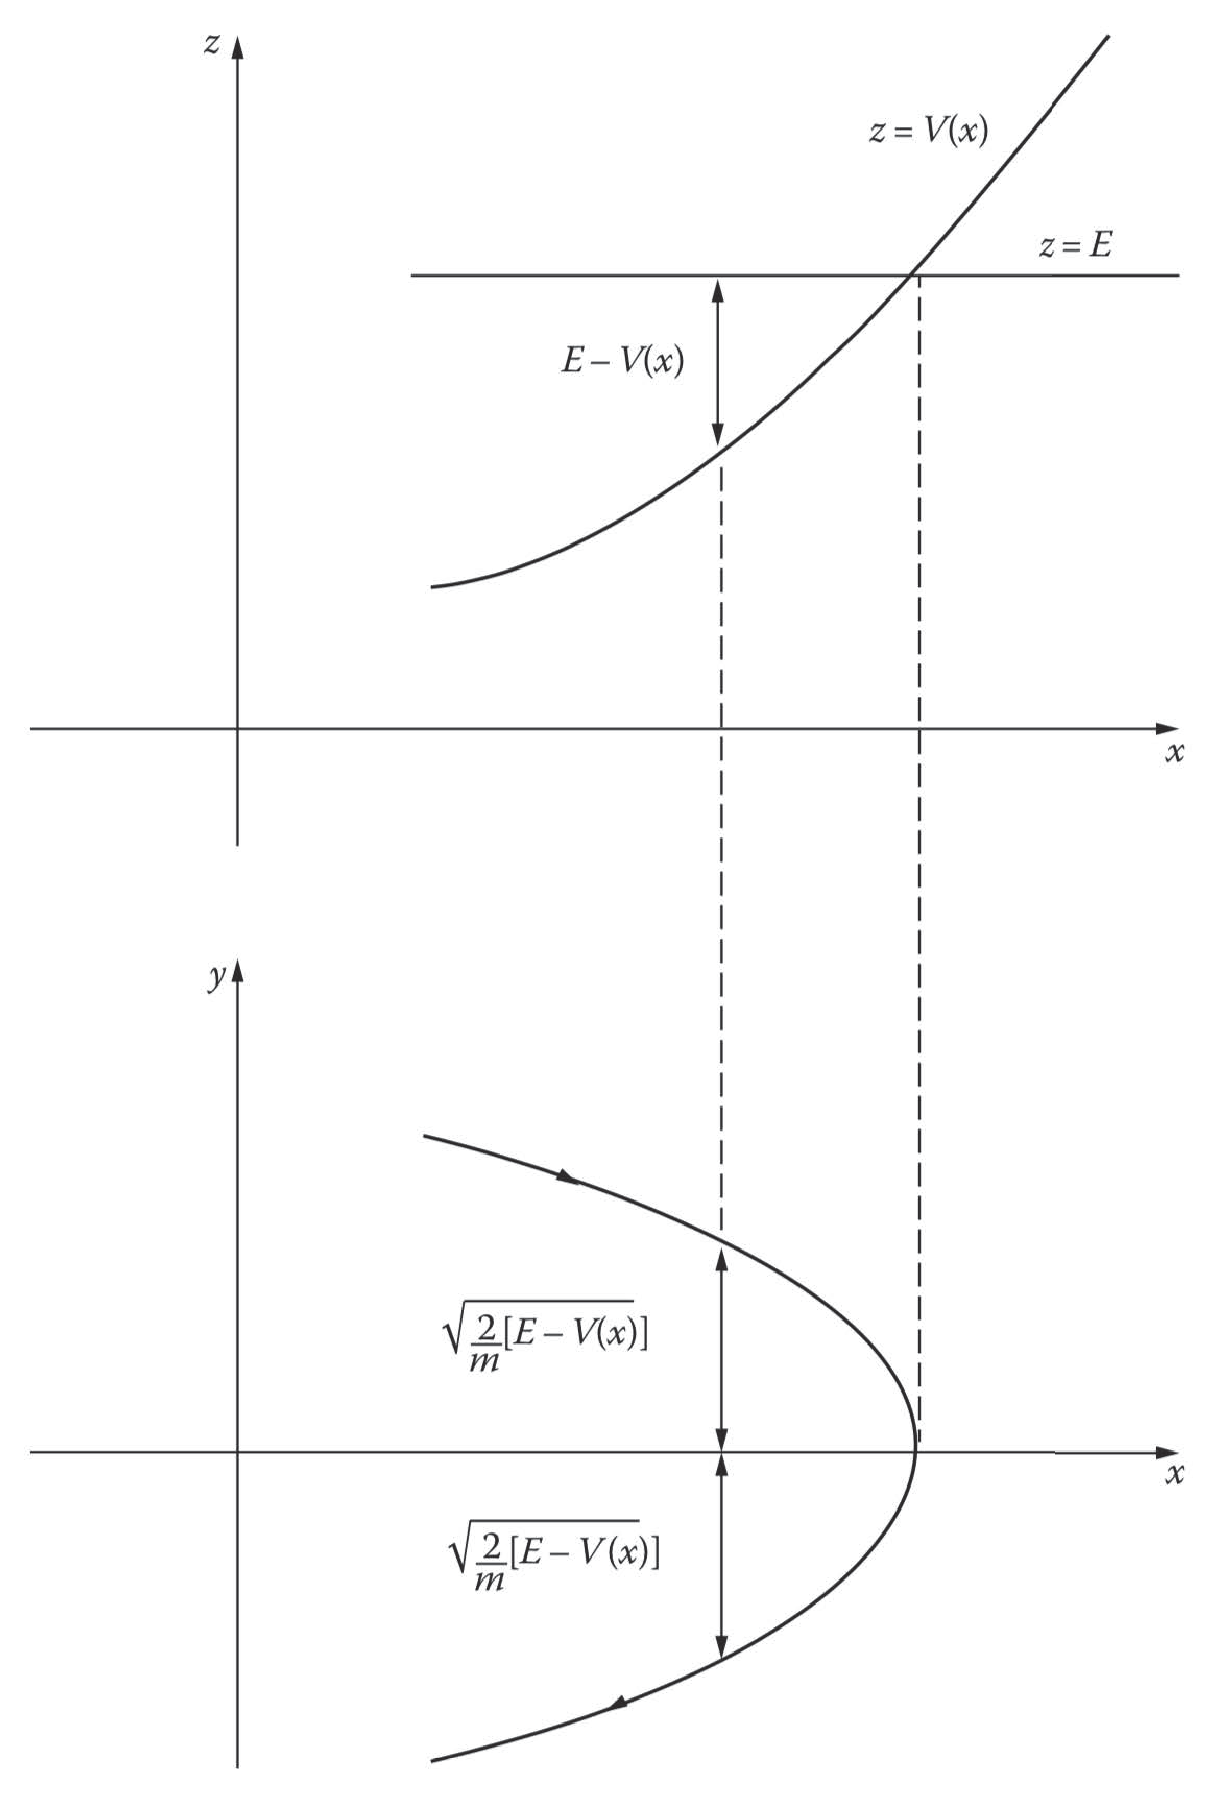
\includegraphics[height=14.cm, angle=0]{nonlinear_conser.eps}
\caption{
}
\label{fig:nonlinear_conser}
\end{figure*}
%===========================================================================================================================

The equation of motion of an undamped pendulum is
\begin{equation}
\dfrac{\dif^2 x}{\dif t^2}  + k \sin x = 0 ~,
\label{eq:pendulum}
\end{equation}
where $k$ is a positive constant. Since this equation is of the form (\ref{eq:nonlinear_con}), it can be interpreted as describing the undamped rectilinear motion of a unit mass under the influence of a nonlinear spring whose restoring force is $-k \sin x$. The autonomous system equivalent is
\begin{equation}
\left\{
\begin{aligned}
\dfrac{\dif x}{\dif t} & =  y \\
\dfrac{\dif y}{\dif t} & =  -k \sin x ~, 
\end{aligned}
\right.
\end{equation}
and its critical points are $(0,0)$, $(\pm \pi,0)$, $(\pm 2\pi,0), \cdots$. The differential equation of the paths is
\begin{equation*}
\dfrac{\dif y}{\dif x}  = -\dfrac{k\sin x}{y} ~,
\end{equation*}
and by separating variables and integrating, the equation of the family of paths is
\begin{align*}
& \dfrac{1}{2}  y^2 + (k-k\cos x) = E ~, \\
& V(x) = \int_0^x f(x) \dif x = k - k\cos x ~.
\end{align*}
Construct the paths by first drawing the graph of $z=V(x)$ and several lines $z=E$ in the $xz$-plane (Figure \ref{fig:phase_pendulum}, where $z = E = 2k$ is the only line shown). From this we read off the values $E - V(x)$ and sketch the paths in the phase plane directly below by using $y = \pm \sqrt{2[E - V(x)]}$. It is clear from this phase portrait that if the total energy $E$ is between $0$ and $2k$, then the corresponding paths are closed and equation (\ref{eq:pendulum}) has periodic solutions. If $E > 2k$, then the path is not closed and the corresponding solution of (\ref{eq:pendulum}) is not periodic. The value $E = 2k$ separates the two types of motion, and for this reason a path corresponding to $E=2k$ is called a \textcolor{red}{separatrix}. The wavy paths outside the separatrices correspond to whirling motions of the pendulum, and the closed paths inside to oscillatory motions. It is evident that the critical points are alternately unstable saddle points and stable but not asymptotically stable centers. Consider the effect of transforming this conservative dynamical system into a nonconservative system by introducing a linear damping force. The equation of motion then takes the form
\begin{equation}
\dfrac{\dif^2 x}{\dif t^2}  +c\dfrac{\dif x}{\dif t}  + k \sin x = 0 ~, ~~~ c > 0 ~,
\end{equation}
and the configuration of the paths is suggested in Figure \ref{fig:phase_pendulum2}. The centers in Figure \ref{fig:phase_pendulum} become asymptotically stable spirals, and also that every path- except the separatrices entering the saddle points as $t \rightarrow \infty$ ultimately winds into one of these spirals.

%===========================================================================================================================
\begin{figure*}
\centering
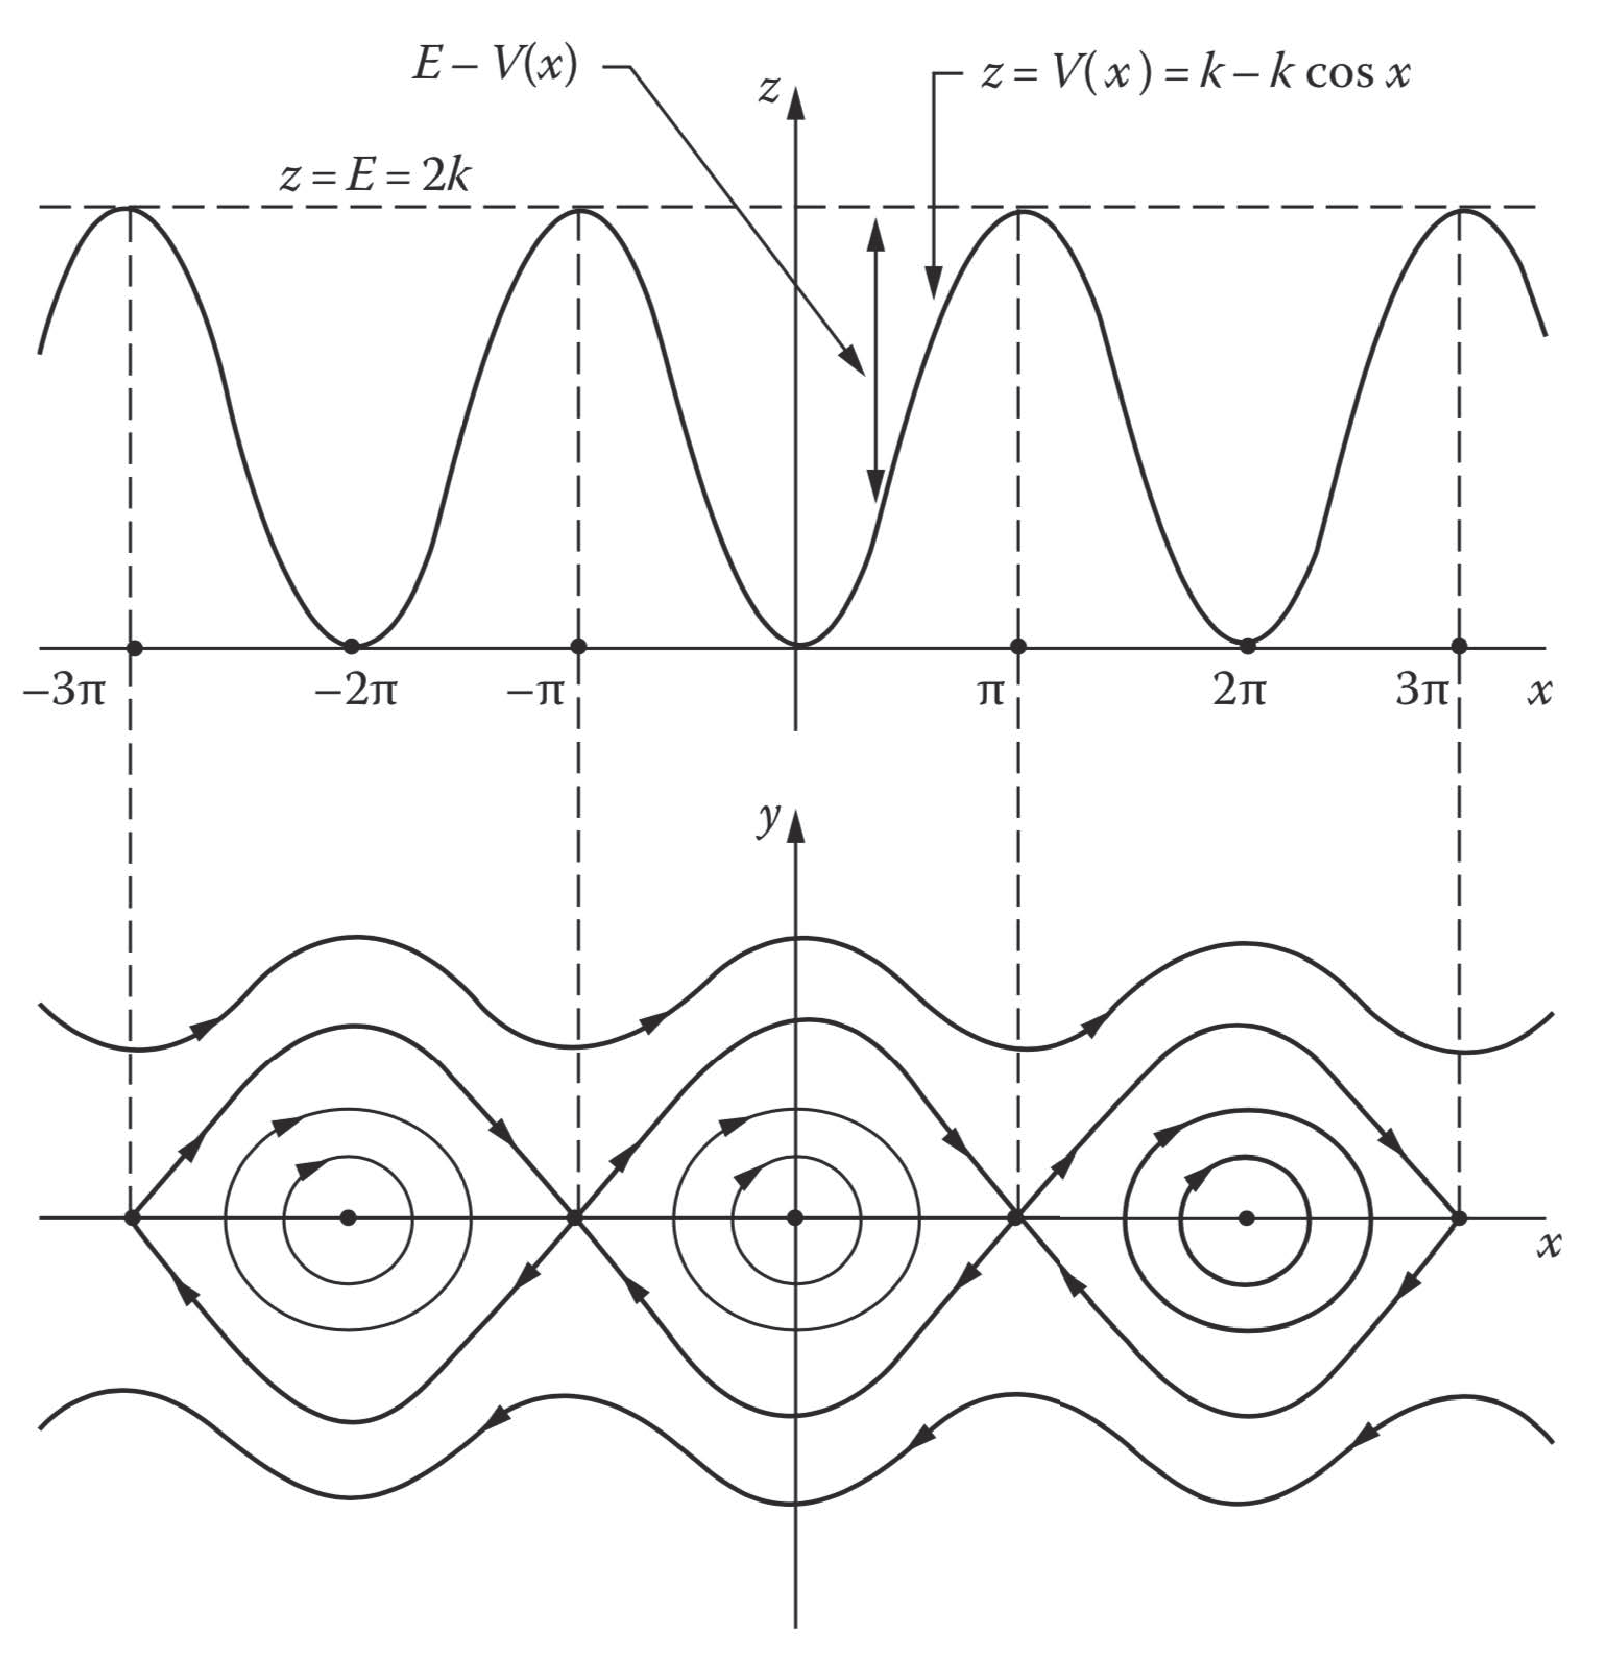
\includegraphics[height=14.cm, angle=0]{phase_pendulum.eps}
\caption{
}
\label{fig:phase_pendulum}
\end{figure*}
%===========================================================================================================================

%===========================================================================================================================
\begin{figure*}
\centering
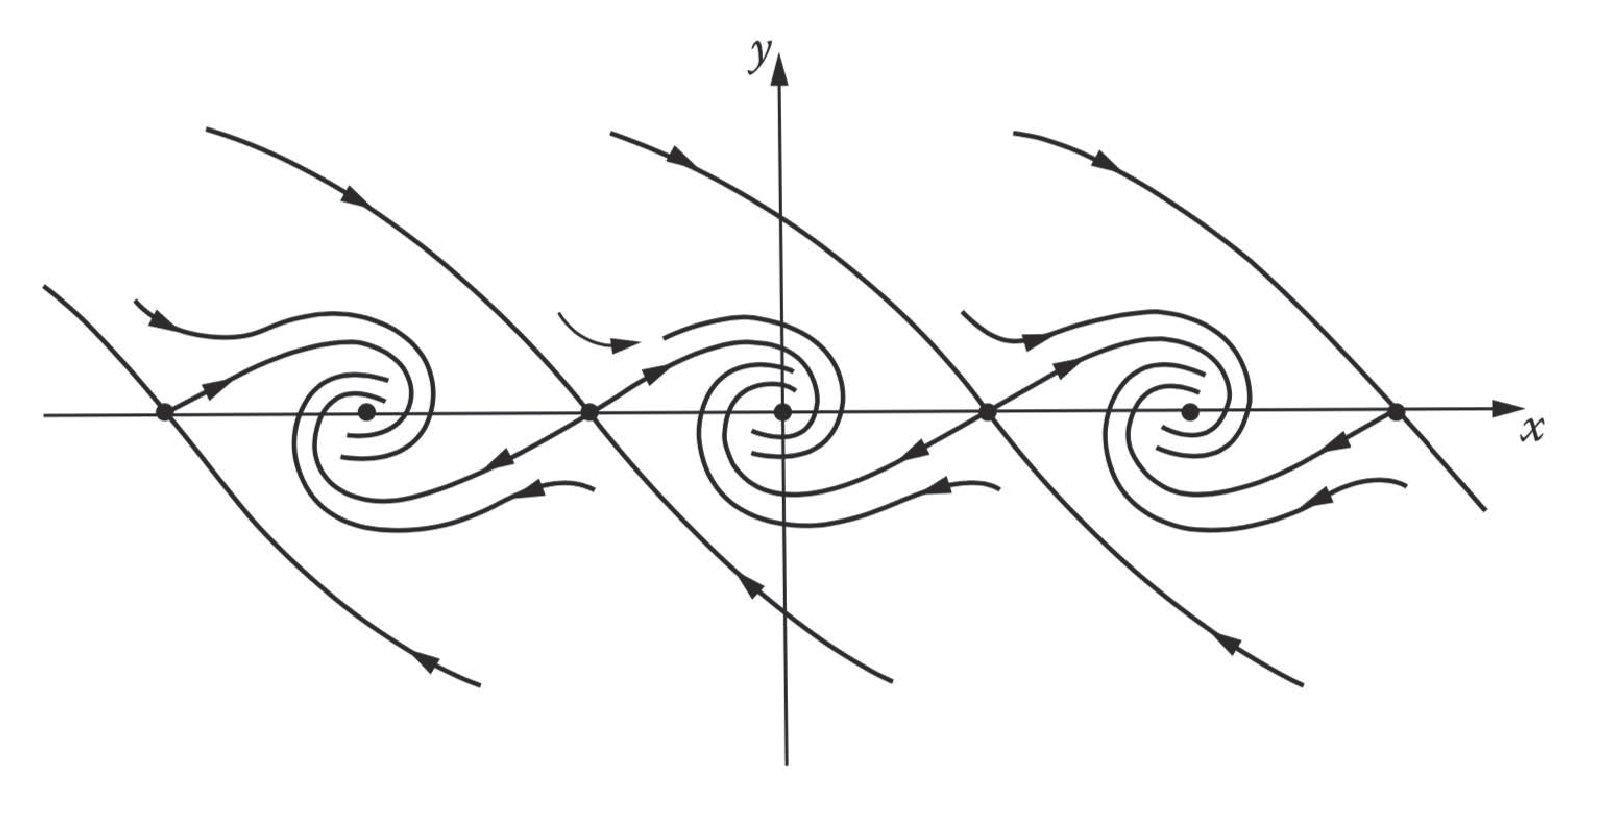
\includegraphics[height=8.cm, angle=0]{phase_pendulum2.eps}
\caption{
}
\label{fig:phase_pendulum2}
\end{figure*}
%===========================================================================================================================









\section{Periodic Solutions. The Poincar\'e-Bendixson Theorem}
\cite{george1991differential, simmons2016differential} Consider a nonlinear autonomous system
\begin{equation}
\left\{
\begin{aligned}
\dfrac{\dif x}{\dif t} & =  F(x,y) \\
\dfrac{\dif y}{\dif t} & =  G(x, y) ~.
\end{aligned}
\right.
\label{eq:nonlinear_gen}
\end{equation}
in which the functions $F(x,y)$ and $G(x,y)$ are continuous and have continuous first partial derivatives throughout the phase plane. 

\begin{tcolorbox}[colback=green!5,colframe=green!40!black,title= Theorem A]
A closed path of the system (\ref{eq:nonlinear_gen}) necessarily surrounds at least one critical point of this system
\end{tcolorbox}



\begin{tcolorbox}[colback=green!5,colframe=green!40!black,title= Theorem B]
If $\partial F/\partial x+\partial G/\partial y$ is always positive or always negative in a certain region of the phase plane, then the system (\ref{eq:nonlinear_gen}) cannot have closed paths in that region.
\end{tcolorbox}


\begin{tcolorbox}[colback=green!5,colframe=green!40!black,title= Theorem C]
Let $R$ be a bounded region of the phase plane together with its boundary, and assume that $R$ does not contain any critical points of the system (\ref{eq:nonlinear_gen}). If $C=[x(t),y(t)]$ is a path of (\ref{eq:nonlinear_gen}) that lies in $R$ for some $t_0$ and remains in $R$ for all $t > t_0$, then $C$ is either itself a closed path or it spirals toward a closed path as $t \rightarrow \infty$. Thus in either case the system (\ref{eq:nonlinear_gen}) has a closed path in $R$.
\end{tcolorbox}

The Poincar\'e-Bendixson theorem is quite satisfying from a theoretical point of view, but in general it is rather difficult to apply. A more practical criterion has been developed that assures the existence of closed paths for equations of the form
\begin{equation}
\dfrac{\dif^2 x}{\dif t^2} +f(x) \dfrac{\dif x}{\dif t} +g(x) = 0 ~,
\label{eq:Lienard}
\end{equation}
which is called \textcolor{red}{Li\'enard's equation}. The equivalent system is
\begin{equation}
\left\{
\begin{aligned}
\dfrac{\dif x}{\dif t} & = y \\
\dfrac{\dif y}{\dif t} & = -g(x) -f(x) y ~.
\label{eq:Lienard_sys}
\end{aligned}
\right.
\end{equation}
and a closed path of (\ref{eq:Lienard_sys}) corresponds to a periodic solution of (\ref{eq:Lienard}). The fundamental statement about the closed paths of (\ref{eq:Lienard}) is


\begin{tcolorbox}[colback=green!5,colframe=green!40!black,title= Theorem D (Li\'enard's Theorem) ]
Let the functions $f(x)$ and $g(x)$ satisfy the following conditions: (i) both are continuous and have continuous derivatives for all $x$;
(ii) $g(x)$ is an odd function such that $g(x) > 0$ for $x > 0$, and $f(x)$ is an even function; and (iii) the odd function $F(x) = \int_0^x f(x) \dif x$ has exactly one positive zero at $x=a$, is $0$ negative for $0 < x < a$, is positive and nondecreasing for $x > a$, and $F(x) \rightarrow \infty$ as $x \rightarrow \infty$. Then equation (\ref{eq:Lienard}) has a unique closed path surrounding the origin in the phase plane, and this path is approached spirally by every other path as $t \rightarrow \infty$.
\end{tcolorbox}









\section{More about the van der Pol Equation}
\cite{george1991differential, simmons2016differential} 









\section{Proof of Li\'enard's Theorem}
\cite{george1991differential, simmons2016differential} Consider Li\'enard's equation
\begin{equation}
\dfrac{\dif^2 x}{\dif t^2} +f(x) \dfrac{\dif x}{\dif t} +g(x) = 0 ~,
\label{eq:Proof_L_Theorem}
\end{equation}
and assume that $f(x)$ and $g(x)$ satisfy the following conditions: (i) $f(x)$ and $g(x)$ are continuous and have continuous derivatives; (ii) $g(x)$ is an odd function such that $g(x) > 0$ for $x > 0$, and $f(x)$ is an even function; and (iii) the odd function $F(x) = \int_0^x f(x) \dif x$ has exactly one positive zero at $x=a$, is negative for $0 < x < a$, is positive and nondecreasing for $x > a$, and $F(x) \rightarrow \infty$ as $x \rightarrow \infty$. We shall prove that equation (\ref{eq:Proof_L_Theorem}) has a unique closed path surrounding the origin in the phase plane, and that this path is approached spirally by every other path as $t \rightarrow \infty$.

The system equivalent to (\ref{eq:Proof_L_Theorem}) in the phase plane is
\begin{equation}
\left\{
\begin{aligned}
\dfrac{\dif x}{\dif t} & =  y \\
\dfrac{\dif y}{\dif t} & =  -g(x) -f(x) y ~.
\end{aligned}
\right.
\end{equation}
By condition (i), the basic theorem on the existence and uniqueness of solutions holds. It follows from condition (ii) that $g(0)= 0$ and $g(x) \neq 0$ for $x \neq 0$, so the origin is the only critical point. Also, any closed path must surround the origin. 
\begin{align*}
\dfrac{\dif^2 x}{\dif t^2} +f(x) \dfrac{\dif x}{\dif t} =  \dfrac{\dif}{\dif t} \left\{ \dfrac{\dif x}{\dif t} +\int_0^x f(x)\dif x \right\} = \dfrac{\dif}{\dif t} [ y +F(x) ] ~,
\end{align*}
suggests introducing a new variable,
\begin{equation}
z = y +F(x) ~.
\end{equation}
\begin{equation}
\left\{
\begin{aligned}
\dfrac{\dif x}{\dif t} & =  z -F(x) \\
\dfrac{\dif z}{\dif t} & =  -g(x) ~.
\end{aligned}
\right.
\label{eq:Proof_L_Theorem2}
\end{equation}
in the $xz$-plane. Again we see that the existence and uniqueness theorem holds, that the origin is the only critical point, and that any closed path must surround the origin. The one-to-one correspondence $(x,y) \leftrightarrow (x,z)$ between the points of the two planes is continuous both ways, so closed paths correspond to closed paths and the configurations of the paths in the two planes are qualitatively similar. The differential equation of the paths of (\ref{eq:Proof_L_Theorem2}) is
\begin{equation}
\dfrac{\dif z}{\dif x}  = \dfrac{-g(x)}{z -F(x)} ~.
\end{equation}

%===========================================================================================================================
\begin{figure*}
\centering
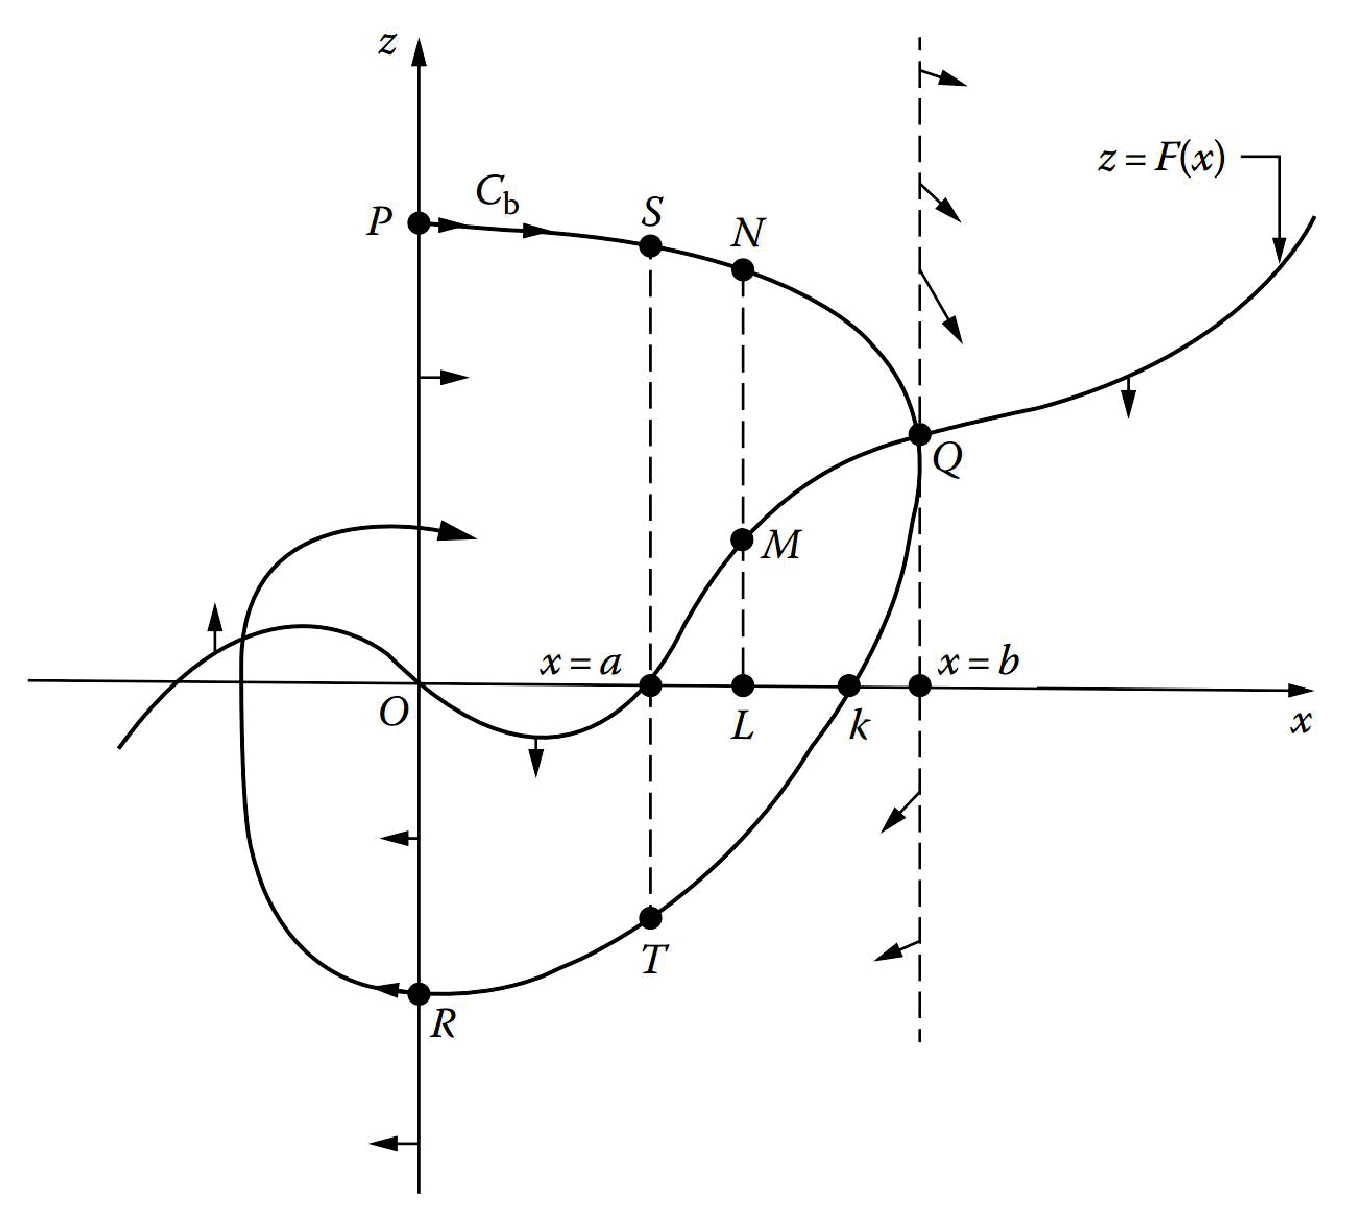
\includegraphics[height=8.cm, angle=0]{Proof_Lienard_ThTheorem.eps}
\caption{
}
\label{fig:Proof_Lienard_ThTheorem}
\end{figure*}
%===========================================================================================================================

Since both $g(x)$ and $F(x)$ are odd, equations (3) and (4) are unchanged when $x$ and $z$ are replaced by $-x$ and $-z$. This means that any curve symmetric to a path with respect to the origin is also a path. Thus if we know the
paths in the right half-plane $(x > 0)$, those in the left half-plane $(x < 0)$ can be obtained at once by reflection through the origin. 

Equation (4) shows that the paths become horizontal only as they cross the $z$-axis, and become vertical only as they cross the curve $z = F(x)$. Also, an inspection of the signs of the right sides of equations (3) shows
that all paths are directed to the right above the curve $z = F(x)$ and to the left below this curve, and move downward or upward according as $x > 0$ or $x < 0$. These remarks mean that the curve $z = F(x)$, the $z$-axis, and the vertical line through any point $Q$ on the right half of the curve $z = F(x)$ can be crossed only in the directions indicated by the arrows. Suppose that the solution of (3) defining the path $C$ through $Q$ is so chosen that the point $Q$ corresponds to the value $t = 0$ of the parameter. Then as $t$ increases into positive values, a point on $C$ with coordinates $x(t)$ and $y(t)$ moves down and to the left until it crosses the $z$-axis at a point $R$; and as $t$ decreases into negative values, the point on $C$ rises to the left until it crosses the $z$-axis at a point $P$. It will be convenient to let $b$ be the abscissa of $Q$ and to denote the path $C$ by $C_b$.

It is easy to see from the symmetry property that when the path $C_b$ is continued beyond $P$ and $R$ into the left half of the plane, the result will be a closed path if and only if the distances $OP$ and $OR$ are equal. To show that there is a unique closed path, it therefore suffices to show that there is a unique value of $b$ with the property that $OP=OR$.

Introduce
\begin{align*}
G(x) &= \int_0^x g(x) \dif x ~, \\
E(x,z) &= \dfrac{1}{2} z^2 +G(x) ~,
\end{align*}
which reduces to $z^2/2$ on the $z$-axis. Along any path
\begin{align*}
\dfrac{\dif E}{\dif x}  = g(x) \dfrac{\dif x}{\dif t} +z \dfrac{\dif z}{\dif t} = -[z-F(x)] \dfrac{\dif z}{\dif t}  +z\dfrac{\dif z}{\dif t}  = F(x) \dfrac{\dif z}{\dif t} ~,
\end{align*}
so
\begin{align*}
\dif E = F \dif z ~.
\end{align*}
If computing the line integral of $F \dif z$ along the path $C_b$ from $P$ to $R$, 
\begin{equation}
I(b) = \int_{PR} F \dif z = \int_{PR} \dif E = E_R -E_P = \dfrac{1}{2}(OR^2 -OP^2) ~,
\end{equation}
so it suffices to show that there is a unique b such that $I(b)=0$.

If $b \leqslant a$, then $F$ and $\dif z$ are negative, so $I(b) > 0$ and $C_b$ cannot be closed. Suppose now that $b > a$. Split $I(b)$ into two parts,
\begin{align*}
I_1(b) &= \int_{PS} F \dif z +\int_{TR} F \dif z ~, \\
I_2(b) &= \int_{ST} F \dif z ~, \\
I(b) &= I_1(b) +I_2(b) ~.
\end{align*}
Since $F$ and $\dif z$ are negative as $C_b$ is traversed from $P$ to $S$ and from $T$ to $R$, it is clear that $I_1(b) > 0$. On the other hand, if we go from $S$ to $T$ along $C_b$ we have $F > 0$ and $\dif z < 0$, so $I_2(b) < 0$. $I(b)$ is a decreasing function of $b$ by separately considering $I_1(b)$ and $I_2(b)$.

Equation (4) enables us to write
\begin{equation*}
F \dif z = F \dfrac{\dif z}{\dif x} \dif x = \dfrac{-g(x) F(x)}{z -F(x)} \dif x ~.
\end{equation*}
The effect of increasing $b$ is to raise the arc $PS$ and to lower the arc $TR$, which decreases the magnitude of $[-g(x)F(x)]/[z - F(x)]$ for a given $x$ between $0$ and $a$. Since the limits of integration for $I_1(b)$ are fixed, the result is a decrease in $I_1(b)$. Furthermore, since $F(x)$ is positive and nondecreasing to the right of $a$, we see
that an increase in $b$ gives rise to an increase in the positive number $-I_2(b)$, and hence to a decrease in $I_2(b)$. Thus $I(b)=I_1(b)+I_2(b)$ is a decreasing function for $b \geqslant a$. $I_2(b) \rightarrow -\infty$ as $b \rightarrow \infty$. If $L$ is fixed and $K$ is to the right of $L$, 
\begin{equation}
I_2(b) = \int_{ST} F\dif z < \int_{NK} f \dif z \leqslant -(LM) \cdot (LN) ~,
\end{equation}
and since $LN  \rightarrow \infty$ as $b  \rightarrow \infty$, $I_2(b)  \rightarrow -\infty$.

$I(b)$ is a decreasing continuous function of $b$ for $b \geqslant a$, $I(a) > 0$, and $I(b) \rightarrow -\infty$ as $b \rightarrow \infty$. It follows that $I(b)=0$ for one and only one $b= b_0$, so there is one and only one closed path $C_{b0}$.

$OR > OP$ for $b < b_0$; and from this and the symmetry we conclude that paths inside $C_{b0}$ spiral out to $C_{b0}$. Similarly, the fact that $OR < OP$ for $b > b_0$ implies that paths outside $C_{b0}$ spiral in to $C_{b0}$.

























































































































%%%%%%%%%%%%%%%%%%%%%%%%%%%%%%%%%%%%%%%%%%%%%%%%%%%%%%%%%%%%%%%%%%%%%%
\bibliographystyle{unsrt_update}
\bibliography{ref}
%%%%%%%%%%%%%%%%%%%%%%%%%%%%%%%%%%%%%%%%%%%%%%%%%%%%%%%%%%%%%%%%%%%%%%

\end{document}